% \documentclass[preprint]{elsarticle}
\documentclass[10pt,conference]{ieeeconf}

% \usepackage{lineno,hyperref}
% \modulolinenumbers[5]

\usepackage{mathrsfs}
\usepackage{graphics} % for pdf, bitmapped graphics files
% \usepackage{epsfig} % for postscript graphics files
\usepackage{amsmath} % assumes amsmath package installed
\usepackage{amssymb}  % assumes amsmath package installed
\let\proof\relax
\let\endproof\relax
\usepackage{amsthm}
\usepackage{cite}
\usepackage{bm}
% \usepackage{subfigure}
\usepackage{acronym}
\usepackage{paralist}
\usepackage{float}
\usepackage{color}
\usepackage{epstopdf}
\usepackage{multicol}
\usepackage{tikz}
\usepackage{hyperref}
% \usepackage{subcaption}
\usepackage{graphicx}
% \usepackage{caption}
\usepackage{soul}
\usepackage{mathtools}
\usepackage{siunitx}
\usepackage{empheq}
\usepackage{accents}
\usepackage{lipsum}
\usepackage{subcaption}
\usepackage{mdframed}
\usepackage[export]{adjustbox}

\makeatletter
\hypersetup{colorlinks=true}
\AtBeginDocument{\@ifpackageloaded{hyperref}
  {\def\@linkcolor{blue}
  \def\@anchorcolor{red}
  \def\@citecolor{red}
  \def\@filecolor{red}
  \def\@urlcolor{red}
  \def\@menucolor{red}
  \def\@pagecolor{red}
\begingroup
  \@makeother\`%
  \@makeother\=%
  \edef\x{%
    \edef\noexpand\x{%
      \endgroup
      \noexpand\toks@{%
        \catcode 96=\noexpand\the\catcode`\noexpand\`\relax
        \catcode 61=\noexpand\the\catcode`\noexpand\=\relax
      }%
    }%
    \noexpand\x
  }%
\x
\@makeother\`
\@makeother\=
}{}}
\makeatother



\newtheorem{Theorem}{Theorem}
\newtheorem{Lemma}{Lemma}
\newtheorem{Problem}{Problem}
\newtheorem{Remark}{Remark}
\newtheorem{Corollary}{Corollary}
\newtheorem{Example}{Example}
\newtheorem{Assumption}{Assumption}
\newtheorem{Definition}{Definition}


\DeclareMathOperator{\rank}{rank}
\DeclareMathOperator{\myspan}{span}
\DeclareMathOperator{\atan2}{atan2}
\DeclareMathOperator{\sgn}{sgn}
\DeclareMathOperator{\sign}{sign}
\DeclareMathOperator{\F}{\mathrm F}
\DeclareMathOperator{\Le}{\mathrm L}
\DeclareMathOperator{\Fp}{\mathrm{F_p}}
\DeclareMathOperator{\R}{\mathbb R}
\DeclareMathOperator{\divergence}{\mathrm{div}}
\DeclareMathOperator{\^T}{^\textrm T}
\DeclareMathOperator{\N}{\textrm N}
\DeclareMathOperator*{\argmax}{arg\,max}
\DeclareMathOperator*{\argmin}{arg\,min}

\newcommand{\bequ}{\begin{eqnarray}}
\newcommand{\eequ}{\end{eqnarray}}
\newcommand{\mT}{^\mathrm{T}}
\newcommand{\rom}{\mathrm}
\def\IR{{\mathbb R}}
\newcommand{\GG}{\text{{\usefont{U}{tx-frak}{m}{n} G}}}
\newcommand{\FF}{\mathcal{F}}
% \newcommand{\SI}{\mathcal{S}}
\newcommand{\LL}{\mathcal{L}}
\newcommand{\ds}{\text{d}s}
\newcommand{\dt}{\text{d}t}
\newcommand{\VV}{\mathcal{V}}
\newcommand{\RI}{\mathcal{R}}
\newcommand{\ubar}[1]{\underaccent{\bar}{#1}}

\IEEEoverridecommandlockouts

\def\BibTeX{{\rm B\kern-.05em{\sc i\kern-.025em b}\kern-.08em
    T\kern-.1667em\lower.7ex\hbox{E}\kern-.125emX}}




\begin{document}

\title{\LARGE \bf An Adaptive Fixed-Time Parameter Estimation and CLF-CBF-QP Control Scheme}
% \title{\LARGE \bf FALCON: a FxTS Adaptation Law for safe CONtrol under parametric model uncertainty}


\author{Mitchell Black \and Ehsan Arabi \and Dimitra Panagou
\thanks{
% This paragraph of the first footnote will contain the date on which you submitted your brief for review. It will also contain support  information, including sponsor and financial support acknowledgment. For  example, ``This work was supported in part by the U.S. Department of  Commerce under Grant BS123456.'' 
The authors would like to acknowledge the support of the National Science Foundation award number 1931982.}
\thanks{The authors are with the Department of Aerospace Engineering, University of Michigan, Ann Arbor, MI, USA; \texttt{\{mblackjr, earabi, dpanagou\}@umich.edu}.}
}
\maketitle

%%%%%%%%%%%%%%%%%%%%%%%%%%%%%%%%%%%%%%%%%%%%%%%%%%%%%%%%%%%%%%%%%%%%%%%%%%%%%%%%
%********************************** Abstract **********************************%
%%%%%%%%%%%%%%%%%%%%%%%%%%%%%%%%%%%%%%%%%%%%%%%%%%%%%%%%%%%%%%%%%%%%%%%%%%%%%%%%

\begin{abstract}
We present a novel technique for solving the problem of safe control for a general class of nonlinear, control-affine systems subject to parametric model uncertainty. Invoking Lyapunov analysis and the notion of fixed-time stability (FxTS), we introduce a parameter adaptation law which guarantees convergence of the estimates of the unknown parameters in the system dynamics to their true values within a fixed-time that is independent of the initial parameter estimation error. We then synthesize the adaptation law with a robust, adaptive control barrier function (RaCBF) based quadratic program to compute safe control inputs despite the considered model uncertainty. For demonstration purposes, we undertake a comparative case study on the efficacy of this result versus other recent approaches to safe control under uncertainty in the literature, and close by highlighting the value of our proposed method in the context of an automobile overtaking another vehicle in a highway scenario.
\end{abstract}


%%%%%%%%%%%%%%%%%%%%%%%%%%%%%%%%%%%%%%%%%%%%%%%%%%%%%%%%%%%%%%%%%%%%%%%%%%%%%%%%
%******************************** Introduction ********************************%
%%%%%%%%%%%%%%%%%%%%%%%%%%%%%%%%%%%%%%%%%%%%%%%%%%%%%%%%%%%%%%%%%%%%%%%%%%%%%%%%

\section{Introduction}

{\color{red} Introduction is incomplete still very much a work in progress. }

How do control engineers design safe, effective controllers for real-world systems if perfect models exist only in their dreams? They must be adept at control design in the presence of uncertainty, which comes in many forms... 

In the context of safety-critical systems represented by \eqref{uncertain system}, obtaining an estimate of $\theta$ that facilitates the satisfaction of forward invariance is of extreme importance for safe control design. Current approaches involve synthesizing parameter estimation laws with aCBF's and RaCBF's in order to perform QP-based control design which renders a safe set forward-invariant \cite{Taylor2019aCBF,Lopez2020racbf}, as well as learning-based techniques \cite{,}. No such method, however, has addressed the issue of convergence of the parameter estimates to a neighborhood of their true values in fixed-time. As motivation, recent advances in safety-critical control for dynamical systems with uncertainty have relied on overly conservative considerations of the effects of such uncertainty. In \cite{black2020quadratic}, the authors design a safe controller while considering that a non-vanishing disturbance on the system dynamics assumes its worst-case, upper bound at all times. In this paper, we seek to improve controller performance, as characterized by the ability of the system trajectories to satisfy specific spatiotemporal objectives, by relaxing worst-case disturbance considerations via an estimate on the modelling error bound in real-time.

The paper is organized as follows. Section II introduces the foundations for Set Invariance, including robust, adaptive control barrier functions (RaCBFs), as well as Finite- and Fixed-Time Stability (FTS, FxTS) and a related FTS parameter adaptation scheme from the literature. In Section III we formalize the problem at hand, while Section IV contains the main results in the form of our novel FxTS adaptation law and its implications on safe control under uncertainty. Sections V and VI highlight a simple, illustrative case study used to compare other recent work to our proposed method and its application on a highway overtake example respectively. We conclude with a summary of contributions and directions for future work in Section VII.


%%%%%%%%%%%%%%%%%%%%%%%%%%%%%%%%%%%%%%%%%%%%%%%%%%%%%%%%%%%%%%%%%%%%%%%%%%%%%%%%
%************************* Mathematical Preliminaries *************************%
%%%%%%%%%%%%%%%%%%%%%%%%%%%%%%%%%%%%%%%%%%%%%%%%%%%%%%%%%%%%%%%%%%%%%%%%%%%%%%%%


\section{Mathematical Preliminaries}\label{sec: math prelim}

In the rest of the paper, $\mathbb R$ denotes the set of real numbers and $\mathbb{R}_{\ge 0}$ the set of non-negative real numbers. We use $\|\cdot\|$ to denote the Euclidean norm and $\|\cdot\|_{\infty}$ to denote the $\mathscr{L}_{\infty}$ norm. As convention, we denote the minimum and maximum eigenvalue of a matrix $A$ as $\lambda_{min}(A)$ and $\lambda_{max}(A)$ respectively. We write $\partial S$ for the boundary of the closed set $S$, and $\textrm{int}(S)$ for its interior. The Lie derivative of a function $V:\mathbb R^n\rightarrow \mathbb R$ along a vector field $f:\mathbb R^n\rightarrow\mathbb R^n$ at a point $x\in \mathbb R^n$ is denoted as $L_fV(x) \triangleq \frac{\partial V}{\partial x} f(x)$. 

We now review set invariance (including its enforcement via control barrier functions), vector projections, finite- and fixed-time stability, and a finite-time parameter adaptation law from the literature which inspired our fixed-time adaptation law. 

%********** Adaptive Safety

\subsection{Set Invariance}

Let us consider the following general class of nonlinear systems:

% \begin{equation}\label{nonlinear system}
%     \begin{aligned}
%         \dot x(t) &= f(t,x(t),u(t)), \quad x(t_0) = x_0
%     \end{aligned}
% \end{equation}

% \noindent where we assume that the state $x \in \mathbb{R}^n$, the input $u \in \mathbb{R}^m$, and $f:[0,\infty) \times \mathbb{R}^n \times \mathbb{R}^m \rightarrow \mathbb{R}^n$ is piecewise-continuous in $t$ and locally Lipschitz in $x$ and $u$. Assuming also that $u(t)$ is both piecewise continuous and bounded over $t$, and that, without loss of generality, $f(t,0,0) = 0$, i.e. the origin of the unforced system is an equilibrium point, it is well-established that for any initial condition, $x_0$, there exists a maximal time interval, $I(x_0) = [t_0, t_0 + \delta]$, over which a unique solution to \eqref{nonlinear system}, $x(t,x_0)$, exists \cite[Theorem 3.1]{khalil2002nonlinear}. 

\begin{equation}\label{nonlinear system}
    \begin{aligned}
        \dot x(t) &= f(t,x(t)), \quad x(t_0) = x_0
    \end{aligned}
\end{equation}

\noindent where we assume that the state $x \in \mathbb{R}^n$, and $f:[0,\infty) \times \mathbb{R}^n \rightarrow \mathbb{R}^n$ is piecewise-continuous in $t$ and locally Lipschitz in $x$. Assuming also that, without loss of generality, $f(t,0) = 0$, i.e. the origin is an equilibrium point, it is well-established that for any initial condition, $x_0$, there exists a maximal time interval, $I(x_0) = [t_0, t_0 + \delta]$, over which a unique solution to \eqref{nonlinear system}, $x(t,x_0)$, exists \cite[Theorem 3.1]{khalil2002nonlinear}. 

For safety-critical systems, we are interested in whether there exists a set, $S$, for which all solutions to initial conditions belonging to $S$ remain within $S$ for all time in the maximal interval of existence, that is, whether $\forall x_0 \in S$, $x(t) \in S$ $\forall t \in I(x_0)$. Such a set would be referred to as \textit{forward-invariant}, the notion of which constitutes the basis for safety. Let us formally define the set in question as

\begin{subequations}\label{set}
    \begin{align}
        S &= \left \{ x \in \mathbb{R}^n : h(x) \geq 0 \right \}\\
        \partial S &= \left \{ x \in \mathbb{R}^n : h(x) = 0 \right \}\\
        \textrm{int}(S) &= \left \{ x \in \mathbb{R}^n : h(x) > 0 \right \}
    \end{align}
\end{subequations}

\noindent where $h: \mathbb{R}^n \rightarrow \mathbb{R}$ is a continuously differentiable function. Then, the following Lemma, known as Nagumo's Theorem and introduced in \cite{nagumo1942invariance}, provides a necessary and sufficient condition for forward-invariance of set \eqref{set}.

\begin{Lemma}\label{lem forward invariance}
    Given a system of the form \eqref{nonlinear system} and a set $S$ described by \eqref{set}, the set $S$ is forward-invariant over the trajectories of \eqref{nonlinear system} with $x(0) \in S$ if and only if the following condition is met:
    
    \begin{equation}\label{def forward invariance}
        \dot{h} = \frac{\partial h}{\partial x}\dot{x} \geq 0, \quad \forall x \in \partial S
    \end{equation}
\end{Lemma}

\noindent In this paper, we consider the class of nonlinear, control-affine systems subject to parametric uncertainty given as:

% a subclass of systems described by \eqref{nonlinear system}: the nonlinear, control-affine dynamical system subject to parametric uncertainty. This system may be formalized as: 

% Enforcing set invariance is a common approach in the modern literature for guaranteeing safety in the context of the evolution of solutions to a dynamical system.

% We now address the notion of set invariance, and thereby also safety, for the following class of nonlinear, control-affine dynamical system subject to parametric uncertainty:
\begin{equation}\label{uncertain system}
    \begin{aligned}
        \dot x(t) &= f(x(t)) + g(x(t))u(t) + \Delta(x(t)) \theta \\
        x(t_0) &= x_0
    \end{aligned}
\end{equation}
\noindent where $x(t) \in \mathbb{R}^n$ denotes the state, $u(t) \in \mathbb{R}^m$ the control input, and $\theta \in \Theta \subset \mathbb{R}^p$ a set of constant, bounded, unknown parameters. We assume that $f: \mathbb{R}^n \rightarrow \mathbb{R}^n$ and now also $g: \mathbb{R}^n \rightarrow \mathbb{R}^{n \times m}$ are locally Lipschitz, that $\Delta : \mathbb{R}^n \times \mathbb{R}_{\ge 0} \rightarrow \mathbb{R}^{n \times p}$ is a known regressor matrix, and that $f$, $g$, and $\Delta$ are bounded for bounded inputs. The $\Delta(x(t))$ matrix may capture, for example, the effects of sensing or modelling errors on the evolution of the system dynamics, whereas the $\theta$ vector parameterizes such errors. We also define $\hat{\theta}$ as the estimated parameter vector, and $\Tilde{\theta} = \theta - \hat{\theta}$ as the parameter estimation error vector.

\begin{Remark}
    {\color{blue}A form of Nagumo's Theorem \eqref{def forward invariance} can be applied to controlled dynamical systems such as \eqref{uncertain system}. We then say that $S$ may be \textit{rendered} forward-invariant if and only if there exists an admissible control for which $L_fh(x) + L_gh(x)u + L_{\Delta}h(x)\theta \geq 0$, $\forall x \in \partial S$.} 
\end{Remark}

One approach to enforcing that the set $S$ as in \eqref{set} is forward-invariant with respect to the uncertain dynamical system \eqref{uncertain system} is to define a subset $S_r \subset S$ which renders $S$ robustly forward-invariant \cite{Lopez2020racbf}. Before formally defining $S_r$, however, we must make the following assumption.

% define a robustly forward-invariant subset of $S$ \cite{Lopez2020racbf}, which we refer to as $S_r$. Before formally defining $S_r$, however, we must make the following assumption.

% Shortly, we will introduce $S_r$ as a function of the maximum parameter error, $\Tilde{\vartheta} = \Tilde{\theta}_{max}$, where $\Tilde{\theta} = \theta - \hat{\theta}$. However, first, we need the following assumption to hold.

\begin{Assumption}\label{ass bounded parameters}
    % The unknown parameters, $\theta$, belong to a known, compact, convex set, $\Theta$, i.e. $\theta \in \Theta$.
    The set $\Theta$ to which the unknown parameters $\theta$ belong is known, compact, and convex.
\end{Assumption}

\begin{Remark}
    There are two direct consequences of Assumption \ref{ass bounded parameters} worth mentioning immediately. Firstly, all parameter vector estimates, $\hat{\theta}$, may be restricted to the set $\Theta$, that is, $\hat{\theta} \in \Theta$. {\color{blue}Thus, it follows secondly that we may infer an upper bound on the norm of the parameter estimation error, $\Tilde{\theta} = \theta - \hat{\theta}$, as $\|\Tilde{\theta}\|_{\infty} \leq \eta = \sup_{\theta_1,\theta_2 \in \Theta}(\|\theta_1 - \theta_2\|_{\infty})$.}
\end{Remark}

We are now ready to present the definition for the robustly forward-invariant subset, $S_r$, as defined in \cite{Lopez2020racbf}.

\begin{subequations}\label{set robust}
    \begin{align}
        S_r &= \left \{ x \in \mathbb{R}^n : h(x) \geq \frac{1}{2} \boldsymbol{\eta}^T \Gamma ^{-1} \boldsymbol{\eta} \right \}\\
        \partial S_r &= \left \{ x \in \mathbb{R}^n : h(x) = \frac{1}{2} \boldsymbol{\eta}^T \Gamma ^{-1} \boldsymbol{\eta} \right \}\\
        \textrm{int}(S_r) &= \left \{ x \in \mathbb{R}^n : h(x) > \frac{1}{2} \boldsymbol{\eta}^T \Gamma ^{-1} \boldsymbol{\eta} \right \}
    \end{align}
\end{subequations}

\noindent where $\Gamma$ is a constant, admissible, positive-definite matrix and $\boldsymbol{\eta} = [\eta \ldots \eta]^T \in \mathbb{R}^p$. With this under consideration, we introduce the new CBF and its associated condition for forward-invariance of the \textit{shrunken set}, $S_r$, as in \cite{Lopez2020racbf}:

\begin{equation}\label{RaCBF}
    h_r(x,\boldsymbol{\eta}) = h(x) - \frac{1}{2} \boldsymbol{\eta}^T \Gamma ^{-1} \boldsymbol{\eta}
\end{equation}

\noindent {\color{blue} and the sufficient condition which renders $S_r$ forward-invariant is}

\begin{equation}\label{robust forward-invariance}
    \dot{h}_r = \frac{\partial h}{\partial x} \dot{x} - \boldsymbol{\eta}^T \Gamma ^{-1} \dot{\boldsymbol{\eta}} \geq -\alpha (h_r)
\end{equation}

\noindent where $\alpha: [0,a) \rightarrow [0,\infty)$ is some class $K$ function, i.e. strictly increasing where $\alpha(0) = 0$. 

\begin{Remark}
    If $S_r$ defined by \eqref{set robust} is forward-invariant, then $S$ defined by \eqref{set} is forward-invariant. Thus, satisfaction of \eqref{robust forward-invariance} implies that \eqref{def forward invariance} holds.
\end{Remark}

We observe that for a time-invariant parameter estimation error, $\dot{\eta} \equiv 0$, the set-invariance condition \eqref{def forward invariance} is recovered on the boundary $h_r(x,\eta) = 0$, or $h(x) = \frac{1}{2} \boldsymbol{\eta}^T \Gamma ^{-1} \boldsymbol{\eta}$, which is why $S_r$ may be referred to as the \textit{shrunken} set.

% {\color{brown}
% From my understanding, Lopez et al. arrives at their result in the following way:

% \begin{equation}\label{Lopez}
%     \begin{aligned}
%         h(x,\Tilde{\theta}) = h_0(x) - \frac{1}{2} \Tilde{\theta} \Gamma ^{-1} \Tilde{\theta}
%     \end{aligned}
% \end{equation}
% which gives
% \begin{equation}
%     \begin{aligned}
%         \dot{h} = \frac{\partial h_0}{\partial x} \dot{x} + \Tilde{\theta} ^T \Gamma ^{-1} \dot{\hat{\theta}} \\
%     \end{aligned}
% \end{equation}

% where 

% \begin{equation}
%     \begin{aligned}
%         \dot{\hat{\theta}} = \Gamma \Delta (x) \frac{\partial h_0}{\partial x}
%     \end{aligned}
% \end{equation}

% and so they end up with the condition:

% \begin{equation}
%     \begin{aligned}
%         \frac{\partial h_0}{\partial x}\left (f(x) + g(x)u - \Delta (x) \hat{\theta} \right ) \geq -\alpha \left (h_0(x) - \frac{1}{2} \Tilde{\theta} \Gamma ^{-1} \Tilde{\theta} \right )
%     \end{aligned}
% \end{equation}

% where basically instead of using an estimate, $\hat{\theta}$, they impose that the condition must hold for all $\theta \in \Theta$. Although they also have this $\frac{\partial h}{\partial x} \Delta (x) \Gamma (\frac{\partial h}{\partial \theta})^T$ term, and I haven't been able to figure out where that comes from.
% }
{\color{blue}
\subsection{Projections on Convex Sets}
Because we know that $\hat{\theta} \in \Theta$ whenever Assumption \ref{ass bounded parameters} is valid, the following Theorem is important to one of the main results of this paper.

\begin{Theorem}[\hspace{-0.3pt}\cite{Luenberger1969Optimization}]\label{Thm: projection}
    Let $x$ be a vector in a Hilbert space, $H$, and let $K$ be a closed, convex subset of $H$. Then, there is a unique vector $k_0 \in K$ such that
    \begin{equation}
        \|x-k_0\| \leq \|x-k\|, \forall k \in K
    \end{equation}
\end{Theorem}

\noindent The implication is that if a parameter adaptation law results in a $\hat{\theta}$ which does not belong to $\Theta$, we may project it back onto $\Theta$ via the projection operator, $P_{\Theta}\hat{\theta}$.

\begin{Definition}
    The projection, $P_{K}x$, of a vector, $x$, on a convex set, $K$, is the vector in $K$ closest to $x$, i.e.
    \begin{equation}\label{def: projection operator}
        \|x - P_Kx\| = \inf_{y \in K}\|x - y\|
    \end{equation}
\end{Definition}
}

\subsection{Finite- and Fixed-Time Stability}

Having addressed safety in the form of set-invariance, we now turn to performance criteria in the forms of finite-time stability (FTS) and fixed-time stability (FxTS) of an equilibrium point of a nonlinear dynamical system. 

\begin{Definition}[\hspace{-0.3pt}\cite{bhat2000finite}]\label{FTS Def}
    The origin of \eqref{nonlinear system} is finite-time stable (FTS) if the following conditions hold:
    \begin{itemize}
        \item {\color{blue}The origin of \eqref{nonlinear system} is stable in the sense of Lyapunov}
        \item Any solution $x(t,x_0)$ of \eqref{nonlinear system} reaches the origin within finite settling-time, $T(x_0)$, i.e. $x(t,x_0) = 0$, $\forall t \geq T(x_0)$.
    \end{itemize}
\end{Definition}

\begin{Definition}[\hspace{-0.3pt}\cite{polyakov2012nonlinear}]\label{FTS Def}
    The origin of \eqref{nonlinear system} is fixed-time stable (FxTS) if it is globally FTS and any solution $x(t,x_0)$ of \eqref{nonlinear system} reaches the origin within finite settling-time, $T$, independent of $x_0$, i.e. $x(t,x_0) = 0$, $\forall t \geq T$.
\end{Definition}

The authors of \cite{bhat2000finite} and \cite{polyakov2012nonlinear} also derive Lyapunov conditions which guarantee FTS and FxTS of the origin respectively. 

% It is important to review these conditions as the FxTS parameter estimation scheme presented in this paper follows from a FTS parameter estimation scheme introduced by \cite{Na2011nonlinear}.

\begin{Theorem}[\hspace{-0.3pt}\cite{bhat2000finite}]\label{FTS Thm}
Suppose there exists a continuous, positive definite function $V:\mathbb R^n\rightarrow\mathbb R$ such that 
\begin{align}\label{Lyapunov Conditions FTS}
    \dot V(x) \leq -aV(x)^p,
\end{align}
holds along the trajectories of \eqref{nonlinear system} with $a>0$ and $0<p<1$. Then, the origin of \eqref{nonlinear system} is FTS with a settling time $T(x)$, where
\begin{align}\label{T(x) FTS}
    T(x) \leq \frac{1}{a(1-p)} V(x)^{1-p}. 
\end{align}
\end{Theorem}

\begin{Theorem}[\hspace{-0.3pt}\cite{polyakov2012nonlinear}]\label{FxTS Thm}
Suppose there exists a positive definite function $V:\mathbb R^n\rightarrow\mathbb R$ such that 
\begin{align}\label{Lyapunov Conditions FxTS}
    \dot V(x) \leq -aV(x)^p-bV(x)^q,
\end{align}
holds along the trajectories of \eqref{nonlinear system} with $a,b>0$, $0<p<1$ and $q>1$. Then, the origin of \eqref{nonlinear system} is FxTS with a settling time $T \leq T_b$ where
\begin{align}\label{eq: T bound old}
    T_b \leq \frac{1}{a(1-p)} + \frac{1}{b(q-1)}. 
\end{align}
\end{Theorem}




\subsection{Finite-Time Parameter Estimation}

The parameter estimation scheme in the following discussion is predicated on Assumption \ref{ass state and control access}.

\begin{Assumption}\label{ass state and control access}
    The state, $x$, and control input $u$, of \eqref{uncertain system} are accessible for measurement.
\end{Assumption}

% We now revisit the class of nonlinear, control-affine systems with parametric uncertainty described by \eqref{uncertain system}. Recall that the regressor matrix, $\Delta (x)$, is assumed to be known and bounded for bounded $x$. Before making an additional assumption on $\Delta (x)$, we must 

\noindent Let us now review the notion of persistent excitation (PE).

\begin{Definition}[\hspace{-0.3pt}\cite{Bodson1989AdaptiveBook}]\label{Def PE}
    A vector or matrix function, $\phi$, is persistently excited (PE) if there exist $T > 0$, $\epsilon > 0$, such that $\int_{t}^{t+T}\phi (r) \phi ^T (r) dr \geq \epsilon I, \forall t \geq 0$.
\end{Definition}

\noindent Now we may introduce the following assumption on $\Delta (x)$.

\begin{Assumption}\label{ass delta PE}
    The regressor matrix $\Delta (x)$ in \eqref{uncertain system} is persistently excited (PE).%, that is, there exist $T > 0$, $\epsilon > 0$, such that $\int_{t}^{t+T}\Delta (x(r)) \Delta ^T (x(r))) dr \geq \epsilon I, \forall t \geq 0$.
\end{Assumption}

\begin{Remark}
    % While persistence of excitation is a difficult condition to satisfy in practice \cite{something}, we note that positive-definiteness implies persistence of excitation and that, therefore, 
    {\color{red}Positive-definiteness of $\Delta^T\Delta$ is sufficient for $\Delta$ satisfying the PE condition.} 
\end{Remark}

\noindent We now review a FTS parameter estimation scheme which forms the foundation for our FxTS parameter estimation law and was first proposed for nonlinear dynamical systems in \cite{Na2011nonlinear}, and extended for robotic applications in \cite{Na2015robotic}. First, we note that we may re-write \eqref{uncertain system} as:

\begin{equation}\label{Na uncertain system}
    \begin{aligned}
        \dot x(t) &= \varphi (x,u) + \Phi (x,u) \theta \\
    \end{aligned}
\end{equation}

% \noindent where $x$, $u$, and $\theta$ are as in \eqref{uncertain system}, and $\varphi: \mathbb{R}^n \times \mathbb{R}^m \rightarrow \mathbb{R}^n$ and $\Phi: \mathbb{R}^n \times \mathbb{R}^m \rightarrow \mathbb{R}^{n \times p}$ are known and bounded for bounded $x,u$.

\noindent where $\varphi(x,u) = f(x) + g(x)u$ and $\Phi(x,u) = \Delta(x)$.
% Notably, this parameter estimation is achieved sans observer; it does assume access to state variables, although not access to rate measurements. 
The variables $x_f$, $\varphi _f$, and $\Phi _f$ are introduced to filter $x$, $\varphi$, and $\Phi$ respectively. The authors of \cite{Na2011nonlinear} and \cite{Na2015robotic} represent these filters as first-order systems, which are described as follows:

\begin{align}
    k\dot{x}_f + x_f &= x, \quad x_f(0) = 0, \quad \dot{x}_f(0) = 0 \label{xf1} \\
    k\dot{\varphi}_f + \varphi _f &= \varphi, \quad \varphi _f(0) = 0, \quad \dot{\varphi}_f(0) = 0 \label{phif1} \\
    k\dot{\Phi}_f + \Phi _f &= \Phi, \quad \Phi _f(0) = 0, \quad \dot{\Phi}_f(0) = 0 \label{phif2}
\end{align}

% we choose the following second-order representations due to their increased capacity to track complex signals more closely: 

% \begin{equation}\label{Filtering Dynamics}
%     \begin{aligned}
%         k^2 \ddot{x}_f + 2k\dot{x}_f + x_f &= x, \quad x_f(0) = 0, \quad \dot{x}_f(0) = 0 \\
%         k^2 \ddot{\varphi}_f + 2k\dot{\varphi}_f + \varphi _f &= \varphi, \quad \varphi _f(0) = 0, \quad \dot{\varphi}_f(0) = 0 \\
%         k^2 \ddot{\Phi}_f + 2k\dot{\Phi}_f + \Phi _f &= \Phi, \quad \Phi _f(0) = 0, \quad \dot{\Phi}_f(0) = 0 \\
%     \end{aligned}
% \end{equation}

\noindent where $k>0$ is a design parameter. Mimicking the form of the system dynamics, the filtered system dynamics are described by:

\begin{align}\label{Filtered System}
    \dot x_f = \varphi _f + \Phi _f\theta
\end{align}

\noindent which serves as the basis for estimating the unknown parameters, $\theta$. As $x_f$, $\varphi_f$, and $\Phi_f$ approach $x$, $\varphi$, and $\Phi$, it becomes possible to reconstruct the uncertain system dynamics and thereby estimate $\theta$.

We now observe that $\dot{x}_f - \varphi = \Phi _f\theta$. With this in mind, define an auxiliary and integrated regressor matrix $P$ and vector $Q$ as:

\begin{align}
    \dot{P} &= -\ell_e P + \Phi_f ^T \Phi_f, \quad &P(0) &= 0 \label{filter P} \\
    \dot{Q} &= -\ell_e Q + \Phi_f ^T (\dot{x}_f - \varphi_f), \quad &Q(0) &= 0 \label{filter Q} 
\end{align}

\noindent the solutions of which are:

\begin{align}
    P(t) &=\int_{0}^{t} e^{-\mathscr{l}(t-r)}\Phi_f ^T(r) \Phi_f (r) dr \label{sol P} \\
    Q(t) &=\int_{0}^{t} e^{-\mathscr{l}(t-r)}\Phi_f ^T(r) (\dot{x}_f(r)-\varphi_f (r)) dr \label{sol Q}
\end{align}

 \noindent and from which it may be discerned that $Q = P\theta$. As such, define an additional auxiliary vector, $W \in \mathbb{R}^p$, which depends on $P$, $Q$, and the estimated parameter vector, $\hat{\theta}$, as
 
 \begin{equation}\label{filter W}
    W = P\hat{\theta} - Q
\end{equation}
 
 It then suffices to show that by defining the parameter estimation error as $\Tilde{\theta} = \theta - \hat{\theta}$, \eqref{filter W} reduces to $W = -P\Tilde{\theta}$ by substituting $Q=P\theta$. This forms the basis for the proposed FT estimation law in \cite{Na2015robotic}, defined by
 
 \begin{equation}\label{FT estimation law}
     \dot{\hat{\theta}} = -\Gamma \frac{P^TW}{\|W\|}
 \end{equation}
 
 \noindent where $\Gamma$ is a constant, positive definite, gain matrix. FTS convergence of the estimated parameters to their true values is guaranteed by the following result.
 
 \begin{Theorem}[\hspace{-0.3pt}\cite{Na2015robotic}]\label{Thm FT Parameter Estimation}
     For system \eqref{Na uncertain system} with parameter adaptation law \eqref{FT estimation law} and $\lambda_{min} (P) > \sigma > 0$, the parameter estimation error $\Tilde{\theta}$ converges to zero in finite-time $t_a$, satisfying $t_a \leq \|\Tilde{\theta}(0)\|\frac{\lambda _{max}(\Gamma ^{-1})}{\sigma}$.
 \end{Theorem}
 
 In Section \ref{sec: Main Results}, we advance this result by proposing a fixed-time parameter adaptation law suitable for the class of systems described by \eqref{uncertain system}. 
 
%  \noindent For the proof, we direct the interested reader to \cite{Na2015robotic}.

%  \begin{proof}
%     Consider the Lyapunov function $V = \frac{1}{2} \Tilde{\theta}^T \Gamma ^{-1} \Tilde{\theta}$, and recall that $W = -P\Tilde{\theta}$ and $\lambda_{min} (P) > \sigma > 0$. Then, the time-derivative of $V$ is $\dot{V} = -\Tilde{\theta}^T \Gamma ^{-1} \dot{\hat{\theta}} = \Tilde{\theta}^T \frac{P^TW}{\|P\hat{\theta} - Q\|} = -\frac{\Tilde{\theta}^T P^T P \Tilde{\theta}}{\|P\Tilde{\theta}\|} \leq -\|P\Tilde{\theta}\| \leq -\kappa \sqrt{V}$ where $\kappa = \sigma \sqrt{2 / \lambda _{max} (\Gamma ^{-1})}$. Therefore, according to Theorem \ref{FTS Thm}, the convergence of the parameter estimation error, $\Tilde{\theta}$, to zero in finite-time is guaranteed, with an upper bound on convergence time expressed as $t_a \leq 2 \sqrt{V(0)} / \kappa$.
%  \end{proof}


% \subsection{Adaptive CLFs}

% {\color{blue}
% \begin{equation}\label{adaptive CLF}
%     \begin{aligned}
%         \hat{\dot{V}} \leq -c_1 V^{\alpha _1} -c_2 V^{\alpha _2} - (\frac{\partial V}{\partial x}) \Delta (x) \Tilde{\theta}
%     \end{aligned}
% \end{equation}

% where

% \begin{equation}\label{adaptive CLF}
%     \begin{aligned}
%         \hat{\dot{V}} = \frac{\partial V}{\partial x} \left (f(x) + g(x)u - \Delta (x) \hat{\theta} \right )
%     \end{aligned}
% \end{equation}

% }
%%%%%%%%%%%%%%%%%%%%%%%%%%%%%%%%%%%%%%%%%%%%%%%%%%%%%%%%%%%%%%%%%%%%%%%%%%%%%%%%
%**************************** Problem Formulation *****************************%
%%%%%%%%%%%%%%%%%%%%%%%%%%%%%%%%%%%%%%%%%%%%%%%%%%%%%%%%%%%%%%%%%%%%%%%%%%%%%%%%
\section{Problem Formulation}

We now present a formalization of the problem under consideration.

% We seek to design a parameter update law in parallel to a controller such that both convergence of the parameter estimation error to a neighborhood of the true values and convergence of the system trajectories to a goal set occur in fixed-time. The main problem statement is as follows:

\begin{Problem}\label{Problem Statement}
    Consider a nonlinear, control-affine dynamical system subject to parametric uncertainty as in \eqref{uncertain system}. Given that Assumption \ref{ass bounded parameters} holds, design a parameter update law, $\dot{\hat{\theta}}$, and associated controller, $u$, such that the following conditions are satisfied: 
    \begin{enumerate}
        \item The parameter estimation error converges to zero within fixed-time, $T_{\theta}$, i.e. $\Tilde{\theta}(t) \rightarrow 0$ as $t \rightarrow T_{\theta} < \infty$, independent of $\Tilde{\theta}(0)$.%, such that a less conservative estimate of model uncertainty may be used in the design of a safe, fixed-time stable controller.
    % \end{enumerate}
    % And subsequently, design a controller, $u$, such that the following objectives are met:
    % \begin{enumerate}
    % \setcounter{enumi}{1}
        \item The system trajectories remain safe for all time, i.e. $x(t) \in S_s$,  $\forall t \geq t_0$.
        \item The system trajectories converge to a goal set within fixed-time, $T_g$, i.e. $x(t) \in S_g$, $\forall t \geq T_g$.
    \end{enumerate}
\end{Problem}

The following section contains our proposed solution to this problem. 

\section{Main Results}\label{sec: Main Results}

Before introducing one of the main results of the paper, we need to address some modifications made to the filtering scheme outlined in \eqref{xf1}-\eqref{phif2}. In place of the first-order scheme used in \cite{Na2011nonlinear},\cite{Na2015robotic}, we elect to use the following second-order filtering scheme:

\begin{align}
    k_e^2\ddot{x}_f + 2k_e\dot{x}_f + x_f &= x \label{xf1 second} \\
    k_e^2\ddot{\varphi}_f + 2k_e\dot{\varphi}_f + \varphi _f &= \varphi \label{phif1 second} \\
    k_e^2\ddot{\Phi}_f + 2k_e\dot{\Phi}_f +  \Phi _f &= \Phi \label{phif2 second}
\end{align}

\noindent where all initial conditions are zero, i.e. $\beta_f(0) = 0$, $\dot{\beta}_f(0) = 0$, $\ddot{\beta}_f(0) = 0$, $\forall \beta \in \{x,\varphi,\Phi\}$. While this second-order system shares the properties of being stable, strictly proper, and minimum-phase with \eqref{xf1}-\eqref{phif2}, it is also critically damped with a natural frequency of $\omega_n = 1/k_e$. This is a desirable characteristic, as it has been well-established that critically damped systems exhibit the smallest settling time, $t_s$, without oscillations \cite{ROSKILLY2015systemTF}. For example, for a unit step input and $k_e=0.001$, the 2$\%$ settling time is $t_s \approx 5.8\times 10^{-3}$.

We are now ready to introduce one of the main results of the paper, a parameter update law which renders the parameter estimation error fixed-time stable and therefore guarantees convergence of the parameters to their true values within fixed-time.

\subsection{FxTS Adaptation Law}

% \noindent where $c_{1e} > 0$, $c_{2e} > 0$, $0 < \gamma _{1e} < 1$, $\gamma _{2e} > 1$, and $\Gamma > 0$ is a constant, diagonal gain matrix, and $\nu$ takes the following form:

% \begin{equation}\label{Lyapunov Function FxT Parameter Update}
%     \nu = \left(\frac{1}{2}W^T P^{-T} \Gamma ^{-1} P^{-1} W \right)
% \end{equation}

% Thus, we are now able to introduce the following result.

\begin{Theorem}\label{Thm: FxT Parameter Adaptation}
    Given a nonlinear, control-affine system with parametric uncertainty as in \eqref{uncertain system}; the filter described by \eqref{xf1 second}-\eqref{phif1 second}; and the auxiliary matrix P and vectors Q, W from \eqref{filter P}-\eqref{filter W}; under the ensuing adaptation law

    \begin{equation}\label{FxT Estimation Law}
        \dot{\hat{\theta}} = \Gamma W \left(W^T P^{-T} W \right)^{-1} \left(-c_{1e} \nu ^{\gamma _{1e}} - c_{2e} \nu ^{\gamma _{2e}} \right),
    \end{equation}
    where
    \begin{equation}\label{Lyapunov Function FxT Parameter Update}
        \nu = \left(\frac{1}{2}W^T P^{-T} \Gamma ^{-1} P^{-1} W \right),
    \end{equation}
    \begin{equation}\label{parameter convergence time}
        T_{\theta} \leq T_b = \frac{1}{c_{1e} (1 - \gamma _{1e})} + \frac{1}{c_{2e} (\gamma _{2e} - 1)}
    \end{equation}
    
    \noindent and $c_{1e} > 0$, $c_{2e} > 0$, $0 < \gamma _{1e} < 1$, $\gamma _{2e} > 1$, and $\Gamma$ is a constant, positive-definite, gain matrix; the estimated parameters, $\hat{\theta}$, converge to the true parameters, $\theta$, in fixed-time, $T_{\theta}$, i.e.  $\Tilde{\theta} \rightarrow 0$ and $\hat{\theta} \rightarrow \theta$ as $t \rightarrow T_{\theta}$, .
\end{Theorem}

\begin{proof}
Consider the Lyapunov function $V_{\Tilde{\theta}} = \frac{1}{2} \Tilde{\theta}^T \Gamma ^{-1} \Tilde{\theta}$. The time-derivative is $\dot{V}_{\Tilde{\theta}} = -\Tilde{\theta}^T \Gamma ^{-1} \dot{\hat{\theta}}$, since $\dot{\theta} = 0$ and $\dot{\Tilde{\theta}} = \dot{\theta} - \dot{\hat{\theta}}$. Applying the parameter update law \eqref{FxT Estimation Law} yields $\dot{V}_{\Tilde{\theta}} = -\Tilde{\theta} ^T W \left( W^T P^{-T} W\right)^{-1} \left(-c_{1e} \nu ^{\gamma _{1e}} - c_{2e} \nu ^{\gamma _{2e}} \right)$. Then, by substituting $W = -P\Tilde{\theta}$ into \eqref{FxT Estimation Law} and \eqref{Lyapunov Function FxT Parameter Update} we obtain
\begin{align}
    \dot{V}_{\Tilde{\theta}} = -c_{1e} V_{\Tilde{\theta}} ^{\gamma _{1e}} - c_{2e} V_{\Tilde{\theta}} ^{\gamma _{2e}}
\end{align}
This is precisely the form of the FxTS condition \eqref{Lyapunov Conditions FxTS}, which in this case holds along the trajectories of $\dot{\Tilde{\theta}}$ with a settling time of \eqref{parameter convergence time}. Therefore, $\Tilde{\theta}$ converges to the origin and, since $\Tilde{\theta} = \theta - \hat{\theta}$, the estimated parameter vector $\hat{\theta}$ converges to the true parameter vector, $\theta$, within fixed-time, $T_{\theta} \leq T_b$.

% where by observing that $\nu = V$ we have that $\dot{V} = -c_{1e} V ^{\gamma _{1e}} - c_{2e} V ^{\gamma _{2e}}$, which satisfies the FxTS condition of \eqref{Lyapunov Conditions FxTS}. Therefore the parameter estimation error, $\Tilde{\theta}$ converges to zero within fixed-time, $T_{\theta} \leq T_b$.
\end{proof}

Whereas previous works introduce the auxiliary and integrated regressors \eqref{filter P} and \eqref{filter Q} in the design of a parameter adaptation scheme which converges in fixed-time to some bounded set (i.e. \cite{Chen2019FxTadaptationrobotic} for robotic manipulators), \eqref{FxT Estimation Law} guarantees fixed-time convergence of the estimated parameters to their true values. With this knowledge, we derive an expression for the upper bound on the $\mathscr{L}_{\infty}$ norm of the parameter error as a function of time.

\begin{Corollary}\label{Cor: upper bound parameter error}
Let $\Tilde{\theta} = \theta - \hat{\theta}$ be the parameter estimation error vector associated with a nonlinear, control-affine system with parametric uncertainty as in \eqref{uncertain system}.
% , for which it is known that Assumption \ref{ass bounded parameters} is valid. 
If the following conditions hold

    \vspace{5pt}\begin{enumerate}
        \item The estimated parameter update law, $\dot{\hat{\theta}}$, is given by \eqref{FxT Estimation Law}
        \item $u(x(t))$ is any locally Lipschitz controller
        \item $\Gamma$ is constant, positive-definite, and \textbf{diagonal}
        \item $\gamma_{1e} = 1 - \frac{1}{\mu_e}$ and $\gamma_{2e} = 1 + \frac{1}{\mu_e}$ for some $\mu_e > 1$
    \end{enumerate}\vspace{5pt}
then the following expression constitutes an upper bound on $\|\Tilde{\theta}\|_{\infty}, \; \forall t \in [0,T_{\theta})$:

% \begin{equation}\label{err bound}
%     \|\Tilde{\theta}\|_{\infty} \leq \sqrt{M\left ( \sqrt{\frac{c_{2e}}{c_{1e}}} \tan{ \left [ \Xi - \frac{\sqrt{c_{1e}c_{2e}}}{\mu_e}t \right ] } \right )^{\mu_e}} = \eta (t)
% \end{equation}

\begin{align}\label{err bound}
    \|\Tilde{\theta}\|_{\infty} \leq \sqrt{M\left ( \frac{1}{N} \tan{ \left [ \Xi - N\frac{c_{1e}}{\mu_e}t \right ] } \right )^{\mu_e}} = \eta (t), 
\end{align}
where $M =  2 \lambda_{max}(\Gamma)$, $N = \sqrt{\frac{c_{2e}}{c_{1e}}}$, and 
{\color{blue}
\begin{equation}
    \Xi = \tan^{-1}{ \left (\frac{1}{2} N \boldsymbol{\eta}^T(0) \Gamma^{-1} \boldsymbol{\eta}(0)\right )}% \leq \frac{\pi}{2}
\end{equation}
with $\boldsymbol{\eta}$ as in \eqref{set robust} and $T_{\theta}$ bounded from above more tightly as follows:
\begin{equation}\label{tighter t bound}
    T_{\theta} \leq \frac{\mu_e\Xi}{\sqrt{c_{1e}c_{2e}}}
\end{equation}
}

\end{Corollary}

\begin{proof}
    % Given that under Assumption \ref{ass delta PE} 
    We again consider the Lyapunov function $V_{\Tilde{\theta}} = \frac{1}{2}\Tilde{\theta} ^T \Gamma ^{-1} \Tilde{\theta}$. As such, we have $\dot{V}_{\Tilde{\theta}} = -c_{1e}V_{\Tilde{\theta}}^{1-1/\mu} - c_{2e}V_{\Tilde{\theta}}^{1+1/\mu}$.
    % Since the parameter update law \eqref{FxT Estimation Law} has been shown to drive the parameter estimation error to zero in fixed-time, we use the FxTS Lyapunov conditions to impose an upper bound on the time-derivative of $V_{\Tilde{\theta}} = \frac{1}{2}\Tilde{\theta} ^T \Gamma ^{-1} \Tilde{\theta}$ as $\dot{V}_{\Tilde{\theta}} \leq -c_{1e}V_{\Tilde{\theta}}^{1-1/\mu} - c_{2e}V_{\Tilde{\theta}}^{1+1/\mu}$. 
    By rearranging variables and setting $x = V_{\Tilde{\theta}}^{1/\mu}$, we obtain:
    \small{
    \begin{align}
        &\int_{V(0)}^{V(t)} \frac{\mu x^{\mu -1} dx}{-c_{1e}x^{\mu-1}-c_{2e}x^{\mu+1}} =\\ \nonumber &-\frac{\mu}{\sqrt{c_{1e}c_{2e}}}\left [\tan^{-1}\left(\sqrt{\frac{c_{2e}}{c_{1e}}}V_{\Tilde{\theta}}^{1/\mu}(t)\right) -  \tan^{-1}\left(\sqrt{\frac{c_{2e}}{c_{1e}}}V_{\Tilde{\theta}}^{1/{\mu}}(0)\right) \right ] \\ \nonumber &= t
    \end{align}} \normalsize
    This leads to 
    \small{
    \begin{align}\label{eq: error bound derivation}
        \nonumber V_{\Tilde{\theta}}(t) &= \left (\sqrt{\frac{c_{1e}}{c_{2e}}} \tan\left [\tan^{-1}\left(\sqrt{\frac{c_{2e}}{c_{1e}}}V(0)\right) -\frac{\sqrt{c_{1e}c_{2e}}}{\mu}t \right]\right)^{\mu}\\
        &= \left (\frac{1}{N} \tan\left [\tan^{-1}\left(N V(0)\right) -N\frac{c_{1e}}{\mu}t \right]\right)^{\mu}
    \end{align}}\normalsize
    where $V(0) = \frac{1}{2}\Tilde{\theta}(0)^T\Gamma^{-1}\Tilde{\theta}(0) \leq \frac{1}{2}\boldsymbol{\eta}(0)^T\Gamma^{-1}\boldsymbol{\eta}(0)$.
    Then, considering $\Gamma$ is diagonal, we can express $V_{\Tilde{\theta}} = \frac{1}{2}(\Gamma^{-1}_{11}\Tilde{\theta}_1^2 + ... + \Gamma^{-1}_{pp}\Tilde{\theta}_p^2)$, and observe that $\frac{1}{2}\lambda^{-1}_{max}(\Gamma)\|\Tilde{\theta}\|_{\infty}^2 \leq \frac{1}{2}\lambda^{-1}_{max}(\Gamma)\|\Tilde{\theta}\|^2 \leq V_{\Tilde{\theta}}$, from which we recover \eqref{err bound} directly. Then, for $0 \leq t < \frac{\mu}{c_{1e}N}\textrm{tan}^{-1}\left(\frac{1}{2}N\boldsymbol{\eta}^T\Gamma^{-1}\boldsymbol{\eta}\right)$, we have that \eqref{eq: error bound derivation} decreases monotonically 
    to zero. As such, we define $\Xi = \textrm{tan}^{-1} \left(\frac{1}{2}N\boldsymbol{\eta}^T\Gamma^{-1}\boldsymbol{\eta}\right)$ and obtain \eqref{tighter t bound}.
    % By considering $\Tilde{\theta}_i^2 \neq 0, \Tilde{\theta}_j^2 = 0$ $\forall j \in [1,p]\setminus i$, we obtain that 
    % \begin{align}
    %     \Tilde{\theta}_i \leq \sqrt{2 \Gamma_{ii} \left ( \sqrt{\frac{c_2}{c_1}} \tan{ \left [ \Xi - \frac{\sqrt{c_1c_2}}{\mu}t \right ] } \right )^{\mu}} 
    % \end{align}
    % \noindent with $\Xi = \tan^{-1}(\sqrt{\frac{c_2}{c_1}}V(0))$. Thus, the more conservative $L_{\infty}$ norm may be applied such that $\|\Tilde{\theta}\|_{\infty} = \max_{i\in[1,p]}\Tilde{\theta}_i$ and we obtain \eqref{err bound}. 
\end{proof}

\begin{Remark}
    As a consequence of \eqref{err bound}, we may tighten the set of admissible parameters at time $t$ as $\Theta(t) = \{\theta \in \mathbb{R}^p: \; \|\theta - \hat{\theta}(t)\|_{\infty} \leq \eta (t)\}$,  $\forall t \in [0,T_{\theta})$.
\end{Remark}

\begin{Remark}
    Under adaptation law \eqref{FxT Estimation Law} and the premises of Corollary \ref{Cor: upper bound parameter error}, $\|\Tilde{\theta}\|_{\infty} = 0$, $\forall t \geq T_{\theta}$, and thus $\Tilde{\Theta}(t)$ shrinks to $\{0\}$ and $\Theta$ shrinks to $\{\theta\}$ within fixed-time, $T_{\theta}$.
\end{Remark}

We may now formalize the new RaCBF condition for guaranteed forward-invariance of sets $S$ and $S_r$, defined in \eqref{set} and \eqref{set robust} respectively.

{\color{blue}
\begin{Theorem}\label{Thm: Adaptive Safety}
    Let $\boldsymbol{\eta} = [\eta \; \dots \; \eta]^T \in \mathbb{R}^p$ where $\eta = \eta(t)$ is given by \eqref{err bound}. Under the premises for Corollary \ref{Cor: upper bound parameter error}, the following condition is sufficient for guaranteeing the forward-invariance of set $S_r$, i.e. \eqref{set robust}:%, and, by extension, $S$, i.e. \eqref{set}:
    \small{
    \begin{align}\label{RaCBF Condition}
            \sup_{u \in U}\{ L_fh(x) &+ L_gh(x)u + \Psi\} \nonumber \\
            &\geq -\alpha \left(h(x) - \frac{1}{2} \boldsymbol{\eta}^T \Gamma^{-1} \boldsymbol{\eta}) \right) + \mathrm{Tr}(\Gamma^{-1})\eta\dot{\eta}
            % + c_{1e} \nu(\boldsymbol{\eta}) ^{\gamma _{1e}} + c_{2e} \nu(\boldsymbol{\eta}) ^{\gamma _{2e}}\nonumber
    \end{align}}\normalsize
    where
    % \begin{equation}
    %     \begin{aligned}
    %         \frac{\partial h}{\partial x}\dot{x} = L_fh(x) + L_gh(x)u + L_{\Delta}h(x)P_{\Theta}\left[\boldsymbol{\eta} + \hat{\theta}\right]
    %     \end{aligned}
    % \end{equation}
    % and
    \small{
    \begin{align}
    \dot{\eta} &= Z\tan^{\frac{\mu_e}{2}-1}\left(\Xi - N\frac{c_{1e}}{\mu_e}t\right)\sec^{2}\left(\Xi - N\frac{c_{1e}}{\mu_e}t\right)\label{eq: eta dot}\\
        % \nu(\boldsymbol{\eta}) &= \frac{1}{2} \boldsymbol{\eta}^T \Gamma^{-1} \boldsymbol{\eta}\label{sup eta}\\
        % \Psi &= 
        % \begin{bmatrix}
        %         \min\left\{(L_{\Delta}h(x))_1P_{\Theta}(\hat{\theta}_1 - \eta),L_{\Delta}h(x)P_{\Theta}(\hat{\theta}_1 + \eta)\right\}\\
        %         \vdots\\
        %         \min\left\{L_{\Delta}h(x)P_{\Theta}(\hat{\theta}_p - \eta),L_{\Delta}h(x)P_{\Theta}(\hat{\theta}_p + \eta)\right\}
        % \end{bmatrix}\label{eq: safety projection}
        \Psi &= 
        \begin{bmatrix}
                \min\left\{D_1P_{\Theta}(\hat{\theta}_1 - \eta),D_1P_{\Theta}(\hat{\theta}_1 + \eta)\right\}\\
                \vdots\\
                \min\left\{D_pP_{\Theta}(\hat{\theta}_p - \eta),D_pP_{\Theta}(\hat{\theta}_p + \eta)\right\}
        \end{bmatrix}\label{eq: safety projection}
        % \Psi &= \min\left\{L_{\Delta}h(x)P_{\Theta}(\hat{\theta} - \boldsymbol{\eta}),L_{\Delta}h(x)P_{\Theta}(\hat{\theta} + \boldsymbol{\eta})\right\}\label{eq: safety projection}
    \end{align}}\normalsize
    for $Z = -c_{1e}\sqrt{MN^{2-\mu_e}}$, where $D_i$ denotes the $i^{th}$ column of $L_{\Delta}h(x)$ for $i \in \{1,\hdots,p\}$, and $P_{\Theta}$ the vector projection onto $\Theta$, as defined in \eqref{def: projection operator}.
    
\end{Theorem}

\begin{proof}
    With $h_r(x,\boldsymbol{\eta}) = h(x) - \frac{1}{2}\boldsymbol{\eta}^T\Gamma^{-1}\boldsymbol{\eta}$ in \eqref{RaCBF} used to define the set $S_r$ in \eqref{set robust}, we must show that if \eqref{RaCBF Condition} holds then \eqref{robust forward-invariance} is guaranteed to hold and thus \eqref{set robust} is forward-invariant. 
    % if \eqref{robust forward-invariance} holds then $S_r$ is forward-invariant. 
    First, whereas $\dot{x}$ is given by \eqref{uncertain system}, we have that $\dot{\boldsymbol{\eta}} = [\dot{\eta} \hdots \dot{\eta}]^T \in \R^p$ and we obtain \eqref{eq: eta dot} by differentiating \eqref{err bound} in Corollary \ref{Cor: upper bound parameter error}. Since $\Gamma$ is diagonal, we can express $\frac{\partial h_r}{\partial \boldsymbol{\eta}}\dot{\boldsymbol{\eta}} = -\boldsymbol{\eta}^T\Gamma^{-1}\dot{\boldsymbol{\eta}} = -\mathrm{Tr}(\Gamma^{-1})\eta\dot{\eta}$.
    
    We consider first the case where $(\boldsymbol{\eta} + \hat{\theta}) \in \Theta$, for which $P_{\Theta}(\boldsymbol{\eta} + \hat{\theta}) = (\boldsymbol{\eta} + \hat{\theta})$. By \eqref{err bound} we have that $\hat{\theta}_i - \eta \leq \theta_i \leq \hat{\theta}_i + \eta$, $\forall i \in \{1,\hdots,p\}$, where $\Theta$ is convex by Assumption \ref{ass bounded parameters}. Thus, the solution of the following minimization problem represents the worst-case effect of the unknown parameters on safety:
    \begin{equation}\label{eq: min phi}
        \phi^* = \argmin_{\phi \in \Theta} L_{\Delta}h(x)\phi
    \end{equation}
    We observe that this is a constrained linear program. As such, a unique minimizer, $\phi^* = [\phi_1^* \; \hdots \; \phi_p^*]^T$ exists, where $\phi_1^*,\;\hdots\;,\phi_p^*$ are the minimizers of the following $p$ constrained linear programs: 
    \begin{equation}
        \phi_i^* = \argmin_{\hat{\theta}_i - \eta \leq \phi_i \leq \hat{\theta}_i + \eta}D_i\phi_i, \quad \forall i \in \{1,\hdots,p\}
    \end{equation}
    Furthermore, the solutions of constrained linear programs are guaranteed to be on the boundary of the solution domain, which in this case implies that either $\phi_i^* = \hat{\theta}_i - \eta$ or $\phi_i^* = \hat{\theta}_i + \eta$. Thus, we define $\Psi = L_{\Delta}h(x)\phi^*$ and recover \eqref{eq: safety projection} so that $\Psi \leq L_{\Delta}h(x)\theta$, $\forall \theta \in \Theta$. 
    
    For $(\boldsymbol{\eta} + \hat{\theta}) \notin \Theta$, \eqref{eq: min phi} is again solved, but now $P_{\Theta}(\boldsymbol{\eta} + \hat{\theta})$ reduces $\eta$ when necessary to enforce that $\phi \in \Theta$. We again obtain that a unique solution exists and that $\Psi \leq L_{\Delta}h(x)\theta$, $\forall \theta \in \Theta$. 
    
    As such, for both cases we have that $L_fh(x) + L_gh(x)u + \Psi \leq \frac{\partial h}{\partial x}\dot{x}$ and thus \eqref{RaCBF Condition} implies \eqref{robust forward-invariance}, and \eqref{set robust} is forward-invariant.
    
    % projects $(\boldsymbol{\eta} + \hat{\theta})$ back onto $\Theta$ so as to constrain the solutions only the worst possible admissible effect of the unknown parameters on safety, i.e. $\phi \in \Theta$.
    
    % As such, we have that 
    
    
    % $P_{\Theta}(\boldsymbol{\eta} + \hat{\theta})$ simply saturates the constraints on the $p$ constrained linear programs at the boundary of $\Theta$ so that 

    
    % We must now show that the definition of \eqref{eq: safety projection} guarantees that $L_fh(x) + L_gh(x)u + \Psi \leq \frac{\partial h}{\partial x}\dot{x}$. 
    % and consequently $L_fh(x) + L_gh(x)u + \Psi \leq \frac{\partial h}{\partial x}\dot{x}$. 
    
    
    
    % $\Psi = L_{\Delta}h(x)\Phi^* \leq L_{\Delta}h(x)\theta$, $\forall \theta \in \Theta$, and consequently $\sup_{u \in U}\{ L_fh(x) + L_gh(x)u + \Psi\} \geq \frac{\partial h}{\partial x}\dot{x}$. 
    
    % With $h_r(x,\boldsymbol{\eta})$ as in \eqref{RaCBF}, the time derivative is $\dot{h}_r(x,\boldsymbol{\eta}) = \frac{\partial h_r}{\partial x}\dot{x} + \frac{\partial h_r}{\partial \boldsymbol{\eta}}\dot{\boldsymbol{\eta}} = \frac{\partial h}{\partial x}\dot{x} - \boldsymbol{\eta}^T\Gamma^{-1}\dot{\boldsymbol{\eta}}$. Whereas $\dot{x}$ is given by \eqref{uncertain system}, we have that $\dot{\boldsymbol{\eta}} = [\dot{\eta} \hdots \dot{\eta}]^T \in \R^p$ and we obtain \eqref{eq: eta dot} by differentiating \eqref{err bound} in Corollary \ref{Cor: upper bound parameter error}. Since $\Gamma$ is diagonal, we can express $\frac{\partial h_r}{\partial \boldsymbol{\eta}}\dot{\boldsymbol{\eta}} = -\boldsymbol{\eta}^T\Gamma^{-1}\dot{\boldsymbol{\eta}} = \mathrm{Tr}(\Gamma^{-1})\eta\dot{\eta}$. We must now show that 
    
    

    % Consider the function $h_r(x,\theta)$, as in \eqref{RaCBF}. Its time-derivative is $\dot{h}_r(x,\Tilde{\theta}) = \frac{\partial h_r}{\partial x}\dot{x} + \frac{\partial h_r}{\partial \Tilde{\theta}}\dot{\Tilde{\theta}}$, where $\dot{\Tilde{\theta}} = \dot{\theta} - \dot{\hat{\theta}} = -\dot{\hat{\theta}}$, since we assume that $\dot{\theta} = 0$. Substituting the system dynamics from \eqref{uncertain system}, our adaptation law \eqref{FxT Estimation Law}, and applying the robust forward-invariance condition \eqref{robust forward-invariance}, we obtain that $\dot{h}_r(x,\Tilde{\theta}) = L_fh(x) + L_gh(x)u + L_{\Delta}h(x)[\Tilde{\theta}+\hat{\theta}] - c_{1e}\nu^{\gamma_{1e}} - c_{2e}\nu^{\gamma_{2e}}$. Since $\nu \leq \nu(\eta)$ by \eqref{sup eta}, we have that \eqref{RaCBF Condition} is a stronger condition than \eqref{robust forward-invariance}, and therefore guarantees forward invariance of $h_r$, which in turn guarantees forward invariance of $h$.
\end{proof}
}

The use of the projection operator in Theorem \ref{Thm: Adaptive Safety} reduces the conservatism of the approach without compromising the robustness of the forward-invariance condition. How then does the restrictiveness of an RaCBF-based safe controller coupled with our parameter adaptation law \eqref{FxT Estimation Law} compare to other proposed controllers in the literature? This is the subject of the following section.

%%%%%%%%%%%%%%%%%%%%%%%%%%%%%%%%%%%%%%%%%%%%%%%%%%%%%%%%%%%%%%%%%%%%%%%%%%%%%%%%
%**************************** Numerical Case Study ****************************%
%%%%%%%%%%%%%%%%%%%%%%%%%%%%%%%%%%%%%%%%%%%%%%%%%%%%%%%%%%%%%%%%%%%%%%%%%%%%%%%%

% \section{Simulation Results and Discussion}\label{sec: results}
\section{Case Study: Comparing Controllers}\label{sec: case study}

In the first numerical study on our proposed method, we investigate how our approach compares to other recent results in the literature, namely against the parameter adaptation laws from \cite{Taylor2019aCBF}, \cite{Lopez2020racbf}, and \cite{Zhao2020robustQP}, and the worst-case disturbance consideration of \cite{black2020quadratic}. As a tool for comparison, we consider a 2D single-integrator system subject to parametric uncertainty and challenge the controllers to 
safely achieve convergence to the origin while avoiding static elliptical obstacles separated by a small gap. Although simple, this example shares commonalities with complex, real-world problems such as autonomous driving.

\begin{figure}[!ht]
    \centering
        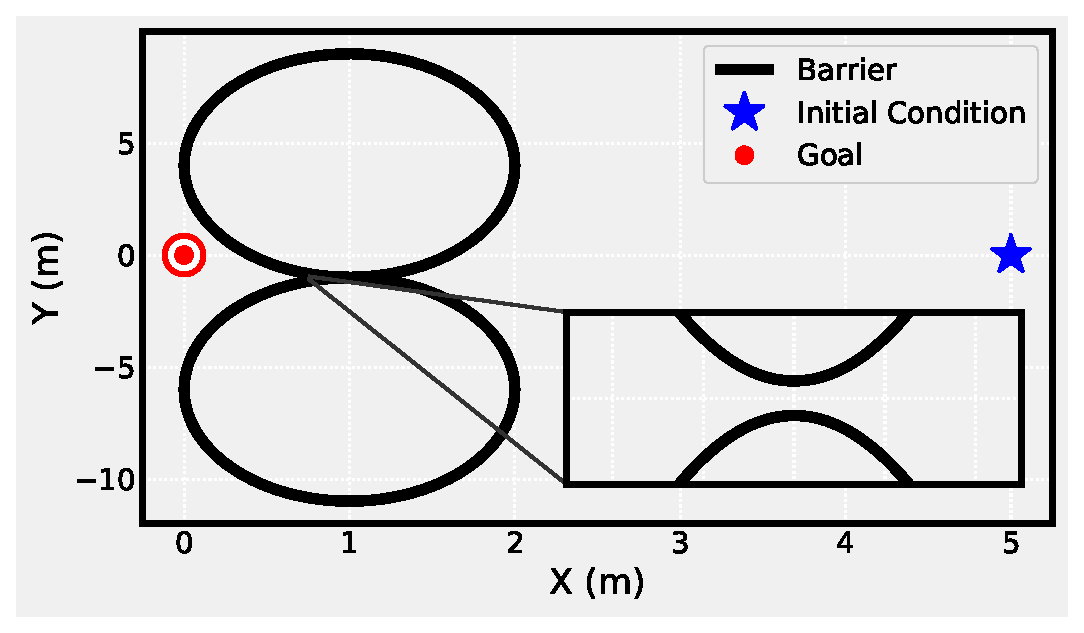
\includegraphics[width=1\columnwidth,clip]{ShootTheGap_ProblemSetup.eps}
    \caption{Problem setup for the first numerical case study, "Shoot the Gap." The controller must determine what actions, $u_x$ and $u_y$, to take in order to realize safe trajectories from the Initial Condition to the Goal.}\label{Fig: Shoot the Gap Setup}
\end{figure}

\subsection{Dynamics}

We denote $z = [x \; y]^T$ as the state, where $x$ and $y$ are the lateral and longitudinal position coordinates as in the Euclidean plane. The system dynamics are described by

\begin{align}\label{eq: simple dynamics}
    \dot{z} &= 
        \begin{bmatrix}
            1 & 0\\
            0 & 1
        \end{bmatrix}
        \begin{bmatrix}
            u_x\\
            u_y
        \end{bmatrix}
        +
        \Delta(z)
        \begin{bmatrix}
            \theta _1\\
            \theta _2
        \end{bmatrix},
\end{align}\normalsize

\noindent where the known regressor matrix is given by

\begin{align}
   \Delta(z) =  \nonumber K_{\Delta}\begin{bmatrix}
            1 + \sin^2(2\pi f_1 x) & 0 \\
            0 & 1 + \cos^2(2\pi f_2 y)
        \end{bmatrix}
\end{align}

\noindent with $\theta_1$, $\theta_2$ as constant parameters which are unknown a priori, and $K_{\Delta}$, $f_1$, $f_2$ given in Table \ref{table simple params}. We enforce that Assumption \ref{ass bounded parameters} holds by defining lower and upper bounds $\ubar{\theta}$ and $\bar{\theta}$ respectively, and imposing $\ubar{\theta} \leq \theta_1,\theta_2 \leq \bar{\theta}$. Notably, the choice of $\Delta$ is such that $\Delta^T\Delta$ positive-definite for all $z \in \R^2$, thus it satisfies the PE condition and Assumption \ref{ass delta PE} holds.

\subsection{Control Formulation}

\begin{figure*}[!ht]
% \begin{mdframed}[backgroundcolor=#1]
\hspace*{-1.25em}
\begin{subfigure}{0.34\linewidth}
    % \centering
    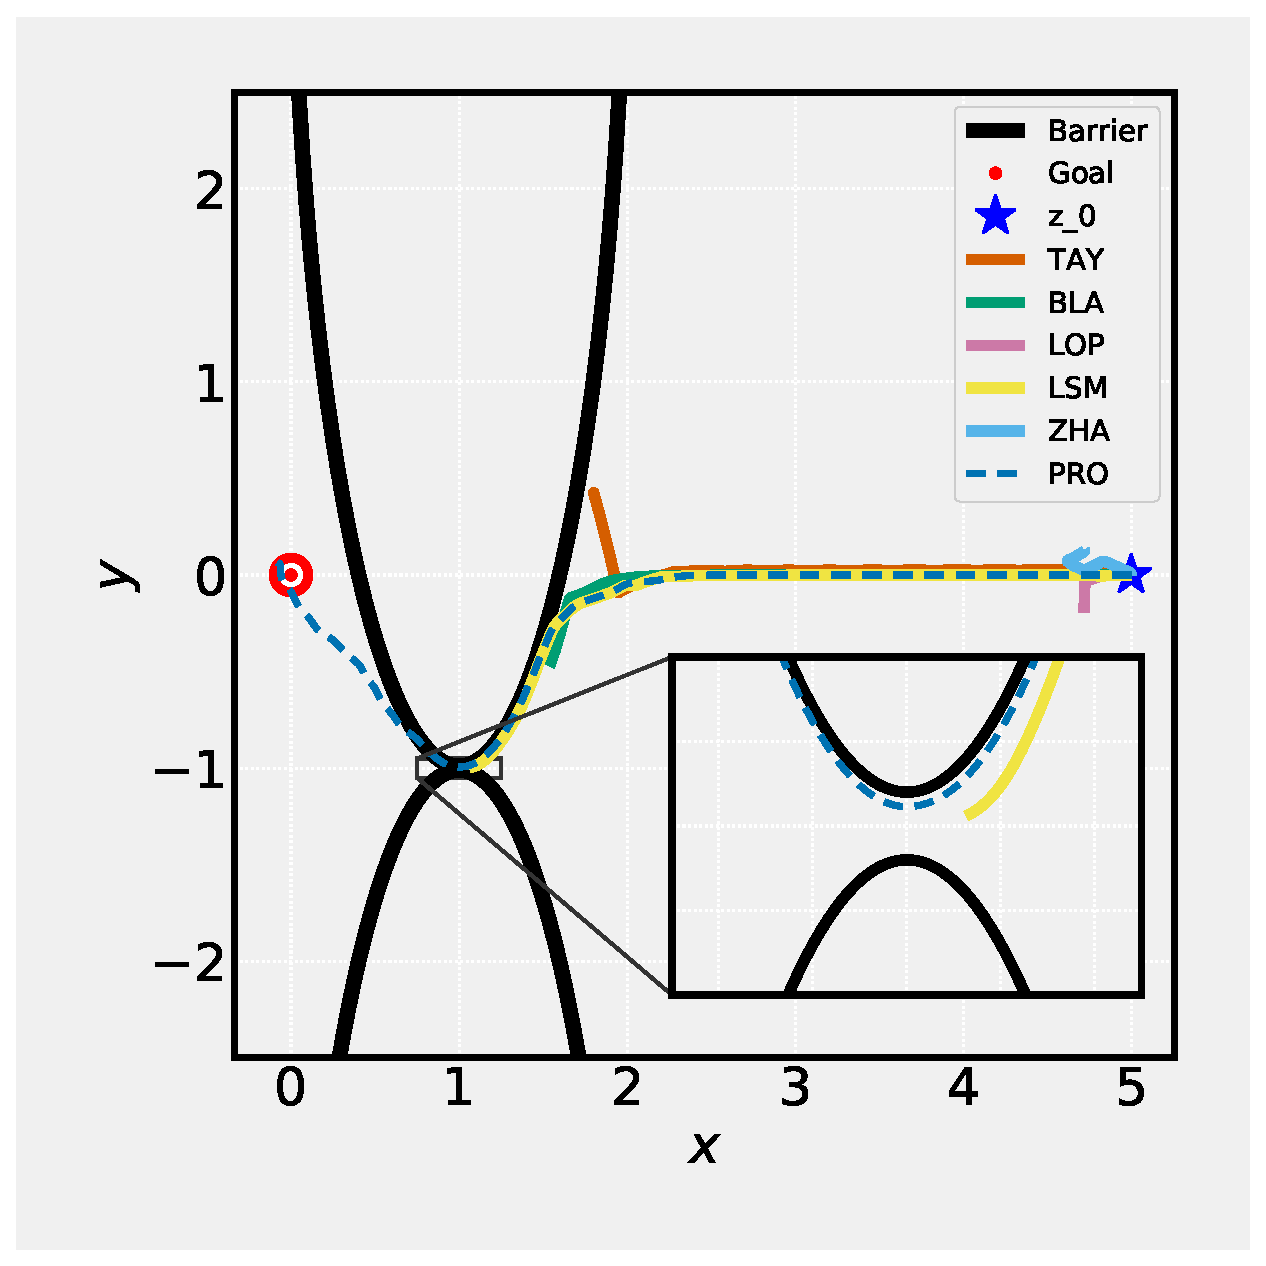
\includegraphics[width=1\textwidth,left]{ShootTheGap_allFxTS_Trajectories_RegX.eps}
    \caption{State trajectories}\label{fig: FxTS shoot the gap - trajectories}
\end{subfigure}%
\hspace*{-0.25em}
\begin{subfigure}{0.34\linewidth}
    % \centering
    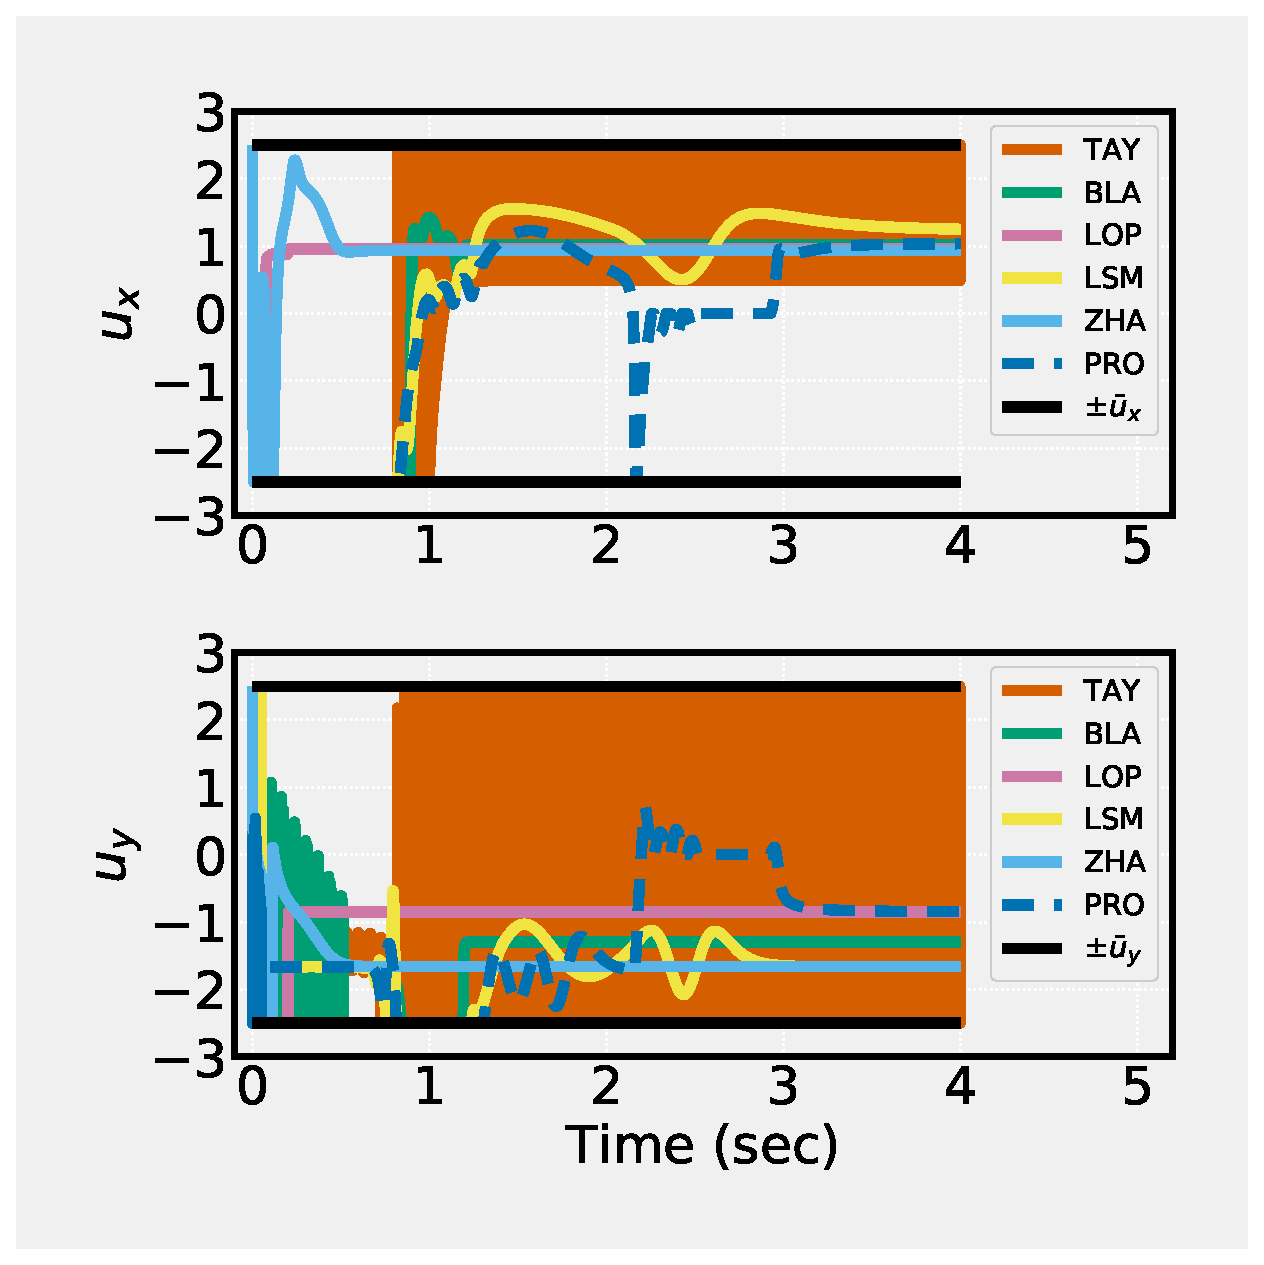
\includegraphics[width=1\textwidth]{ShootTheGap_allFxTS_Controls_RegX.eps}
    \caption{Control inputs}\label{fig: FxTS shoot the gap - controls}
\end{subfigure}%
\hspace*{-0.25em}
\begin{subfigure}{0.34\linewidth}
    % \centering
    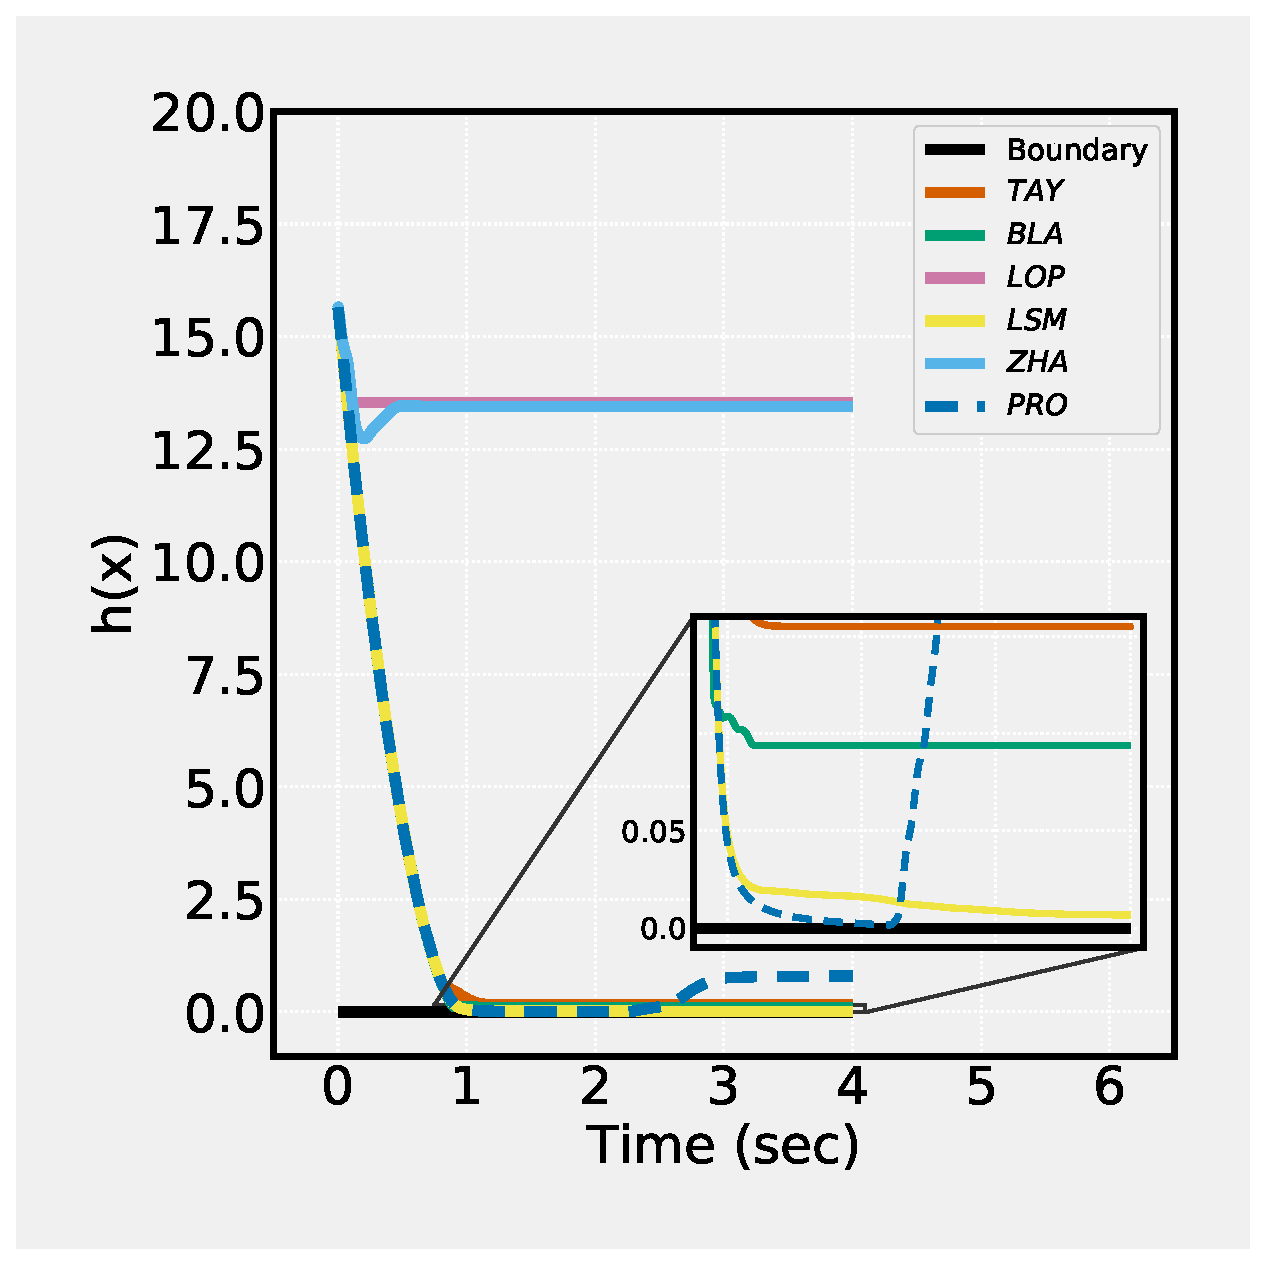
\includegraphics[width=1\textwidth,right]{ShootTheGap_allFxTS_CBFs_RegX.eps}
    \caption{Value of level curve for safe set}\label{fig: FxTS shoot the gap - cbfs}
\end{subfigure}%
\caption{State trajectories, control inputs, and control barrier function evolutions in time for the Shoot the Gap example.}
% \end{mdframed}
\end{figure*}

In order to encode the goal-convergence criterion, we define the following Control Lyapunov Function:

\begin{align}\label{clf simple}
    V(z) = K_V(x^2 + y^2)
\end{align}

\noindent where $K_V>0$ is a design parameter. We define the safe states as those residing outside of the two unsafe ellipses shown in Figure \ref{Fig: Shoot the Gap Setup}, which results in the following two Control Barrier Functions:

\begin{align}\label{cbfs simple}
    h_1(z) = \frac{(x - x_1)^2}{a^2} + \frac{(y - y_1)^2}{b^2} - 1 \\
    h_2(z) = \frac{(x - x_2)^2}{a^2} + \frac{(y - y_2)^2}{b^2} - 1
\end{align}

\noindent where $x_1$, $x_2$, $y_1$, $y_2$, $a$, and $b$ are parameters which define the location, size, and shape of the ellipses. 
% We then have the following RaCBFs:

% \begin{align}\label{racbfs simple}
%     h_{1r}(z,\Tilde{\theta}) = h_1(z) - \frac{1}{2}\Tilde{\theta}^T\Gamma^{-1}\Tilde{\theta} \\
%     h_{2r}(z,\Tilde{\theta}) = h_2(z) - \frac{1}{2}\Tilde{\theta}^T\Gamma^{-1}\Tilde{\theta}
% \end{align}

Due to its demonstrated success (i.e. \cite{ames2012control}, \cite{xu2015robustness}, etc.) in solving for control inputs to performance-aware safety-critical systems, we choose the CLF-CBF-QP framework for control design. While performance objectives are incongruent across the controllers considered from the literature, we have elected to simulate the controllers both in their original form and with standardized CLF constraints in the form of the FxTS conditions \eqref{Lyapunov Conditions FxTS} in order to more fairly assess their abilities to perform safe control under uncertainty. As such, we present our control framework as follows:

\small{
\begin{subequations}\label{CLF-CBF QP}
\begin{align}
    \min_{u,\delta _0,\delta _1,...,\delta_q} \frac{1}{2}u^{T}Qu &+p_0\delta _0^2 + \sum_{i=1}^q p_i\delta _i^2\\ %+p_2\delta _2^2\label{pt_J}\\
    \nonumber &\textrm{s.t.} \\
    -\bar{u}_1 \leq &u_1 \leq \bar{u}_1 \label{ux constraint} \\
    -\bar{u}_2 \leq &u_2 \leq \bar{u}_2 \label{uy constraint} \\ 
    1 &\leq \delta_i \label{d1 constraint} \\
    % 1 &\leq \delta_2 \label{d2 constraint} \\
    \nonumber L_fV(z)+L_gV(z)u&+\phi(x,\Delta(x,t),\hat{\theta},\eta)\\
    \leq  \delta _0 &- c_1V(z)^{\gamma _1} - c_2V(z)^{\gamma _2} \label{pt_V}\\
    L_fh_i(z)+L_gh_i(z)u&+\psi(x,\Delta(x,t),\hat{\theta},\eta) \geq -\delta _ih_i(z) \label{pt_S1}%\\
    % L_fh_2(z)+L_gh_2(z)u&+\psi(x,\Delta(x,t),\hat{\theta},\eta) \geq -\delta _2h_2(z) \label{pt_S2}
\end{align}
\end{subequations}}\normalsize

\noindent $\forall i \in \{1,\hdots,q\}$, where generally $u = [u_1 \; u_2]^T$ and for this problem $u_1=u_x$ and $u_2=u_y$, $\delta_0$ is a relaxation parameter on the performance objective whose inclusion guarantees feasibility of the QP, $\delta_i$ allows for larger negative values of $\dot{h}_i(z)$ away from the boundary of the safe set, and $p_i$ penalizes values of $\delta_i$, $\forall i \in \{0,...,q\}$.
% $\delta_1$ and $\delta_2$ allow for larger negative values of $\dot{h}_1(z)$ and $\dot{h}_2(z)$ away from the boundary of the safe set, and $p_0$, $p_1$, and $p_2$ penalize nonzero values of $\delta _0$, $\delta _1$, and $\delta_2$ respectively. 
The functions $\phi: \mathbb{R}^n \times \mathbb{R}^{n\times p} \times \mathbb{R}^p \times \mathbb{R}^p \rightarrow \mathbb{R}$ and $\psi: \mathbb{R}^n \times \mathbb{R}^{n\times p} \times \mathbb{R}^p \times \mathbb{R}^p \rightarrow \mathbb{R}$ represent the terms specific to the way each respective controller handles the uncertainty in the system dynamics. While all of \eqref{ux constraint}-\eqref{pt_S1} are linear in the decision variables, \eqref{ux constraint} and \eqref{uy constraint} enforce input constraints, \eqref{d1 constraint}
% and \eqref{d2 constraint} 
prevents over-conservatism in enforcing safety, \eqref{pt_V} encodes FxT convergence to the goal, and safety is guaranteed by \eqref{pt_S1}.
% and \eqref{pt_S2}.

\subsection{Problem Setup}

The full set of parameters for this numerical case study are provided in Table \ref{table simple params}.
{\small
\begin{table}[h!]
    \setlength{\tabcolsep}{4pt}
    \centering
    \caption{Shoot the Gap Parameters}\label{table simple params}
    \begin{tabular}{|c|c|c|c|c|c|c|c|c|c|}
        \hline
        $\dot{x}$ & Val & QP & Val & CBF & Val & CLF & Val & $\dot{\hat{\theta}}$ & Val \\ \hline
        $f_1$ & 1  & $Q$ & $I_{2\times2}$ & $a$ & 1 & $K_V$ & 1 & $k_e$ & 0.001 \\ \hline
        $f_2$ & 4 & $p_0$ & 50 & $b$ & 4.99 & $T$ & 4 & $T_e$ & 0.2 \\ \hline
        $\theta_1$ & -1 & $p_1$ & 5 & $x_1$ & 1 & $\mu$ & 5 & $\mu_e$ & 5 \\ \hline
        $\theta_2$ & 1 & $p_2$ & 5  & $x_2$ & 1 & $c_1$ & 1.963 & $c_{1e}$ & 50 \\ \hline
        $K_{\Delta}$ & 0.833 & $\bar{u}_1$ & 2.5 & $y_1$ & -6 & $c_2$ & 1.963 & $c_{2e}$ & 50  \\ \hline
        & & $\bar{u}_2$ & 2.5 & $y_2$ & 4 & $\gamma_1$ & 0.8 & $\gamma_{1e}$ & 0.8  \\ \hline
        & & & & & & $\gamma_2$ & 1.2 & $\gamma_{2e}$ & 1.2 \\ \hline
        & & & & & & & & $\ell_e$ & 100\\
        \hline 
    \end{tabular}
\end{table}}

We endeavor to show that by learning the true values of the uncertain parameters in the system dynamics of \eqref{eq: simple dynamics}, our proposed method is capable of approaching the boundary of the safe set more closely than previous results in the literature and, as a consequence, able to reach a goal which may require such an approach despite such uncertainty. Table \ref{tab: key other works} provides the legend codes used to refer to these other works.

\begin{table}[h!]
    \centering
    \caption{Controllers from the Literature}\label{tab: key other works}
    \begin{tabular}{|c|c|c|c|c|c|c|c|}
        \hline
        Authors & Citation & Legend Code \\ \hline
        Taylor et al. & \cite{Taylor2019aCBF} & TAY \\ \hline
        Black et al. & \cite{black2020quadratic} & BLA \\ \hline
        Lopez et al. & \cite{Lopez2020racbf} (w/o SMID) & LOP \\ \hline
        Lopez et al. & \cite{Lopez2020racbf} (w/ SMID) & LSM \\ \hline
        Zhao et al. & \cite{Zhao2020robustQP} & ZHA \\ \hline
        Proposed Method &  & PRO \\ \hline
    \end{tabular}\par
    \bigskip
    Note: \cite{Lopez2020racbf} presents RaCBF-based control formulations both with and without Set Membership Identification (SMID) as a means to estimate the unknown model parameters. We have considered both in our simulations.
\end{table}

\subsection{Results}

Firstly, we observe that in accordance with Theorem \ref{Thm: FxT Parameter Adaptation}, Figure \ref{fig: theta hats} highlights that the parameter estimates, $\hat{\theta}$, do in fact converge to their true values within fixed-time $T_{\theta}$ given by \eqref{tighter t bound}.

\begin{figure}[!h]
    \centering
        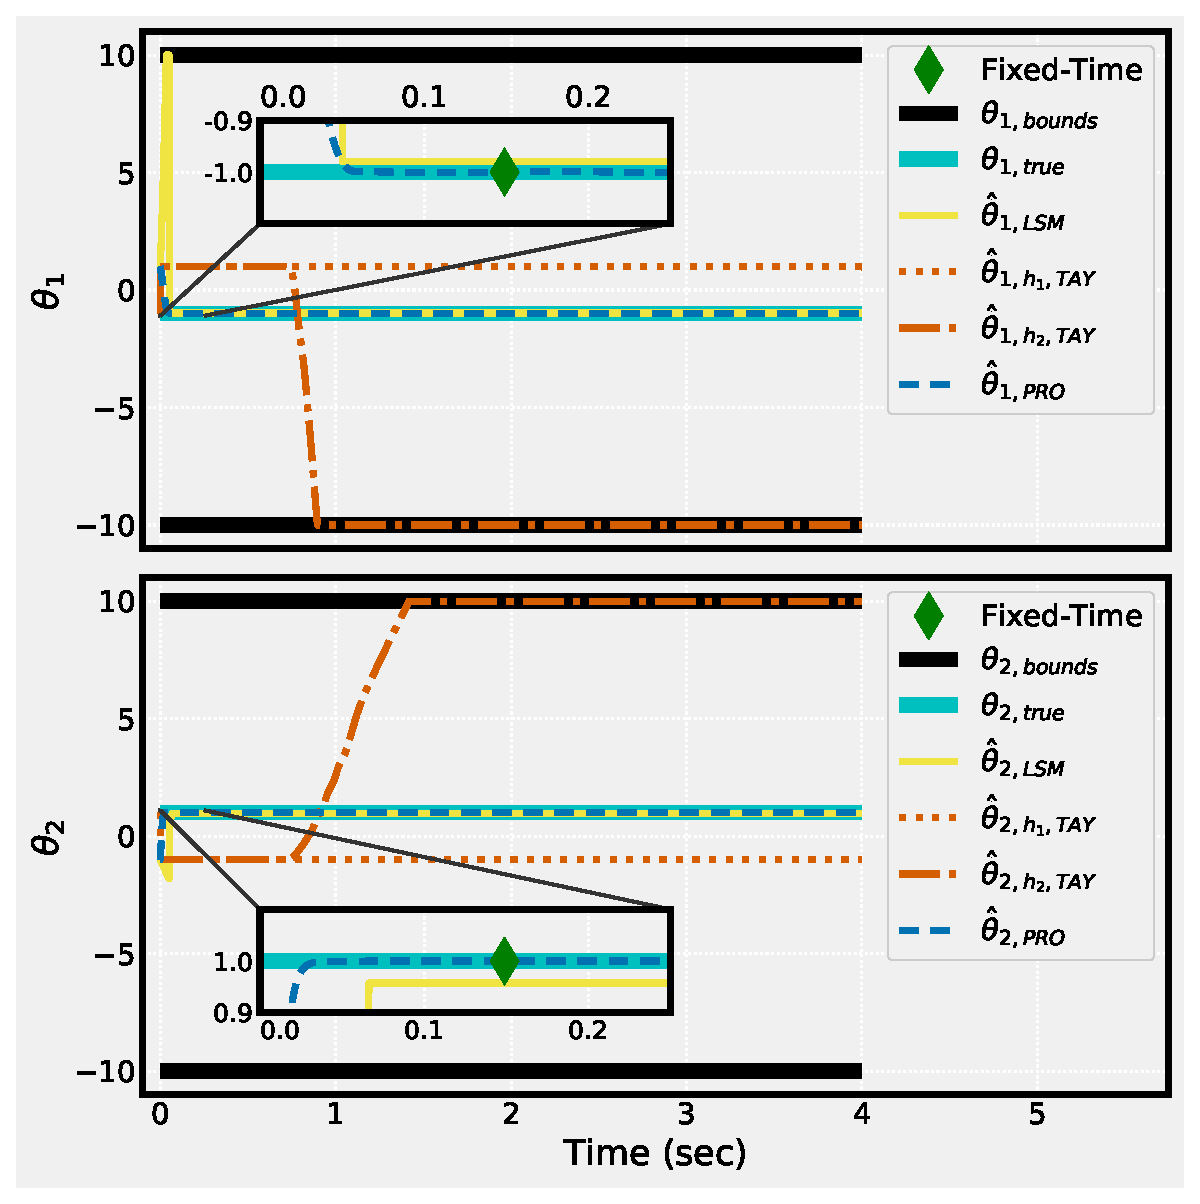
\includegraphics[width=1\columnwidth,clip]{ShootTheGap_ThetaHats_RegX.eps}
    \caption{Evolution of the estimates of the unknown model parameters, $\theta$.}\label{fig: theta hats}
\end{figure}

We observe from Figure \ref{fig: FxTS shoot the gap - trajectories} that our proposed method solves this problem where the other methods do not; that is, our method achieves convergence to the origin within fixed-time because the controller can tolerate regions of the state space which exist in close proximity to the boundary of the safe region. In this sense, our synthesized adaptation law and RaCBF-based controller is less restrictive than the existing literature.

% \begin{figure*}[!ht]
%     \centering
%         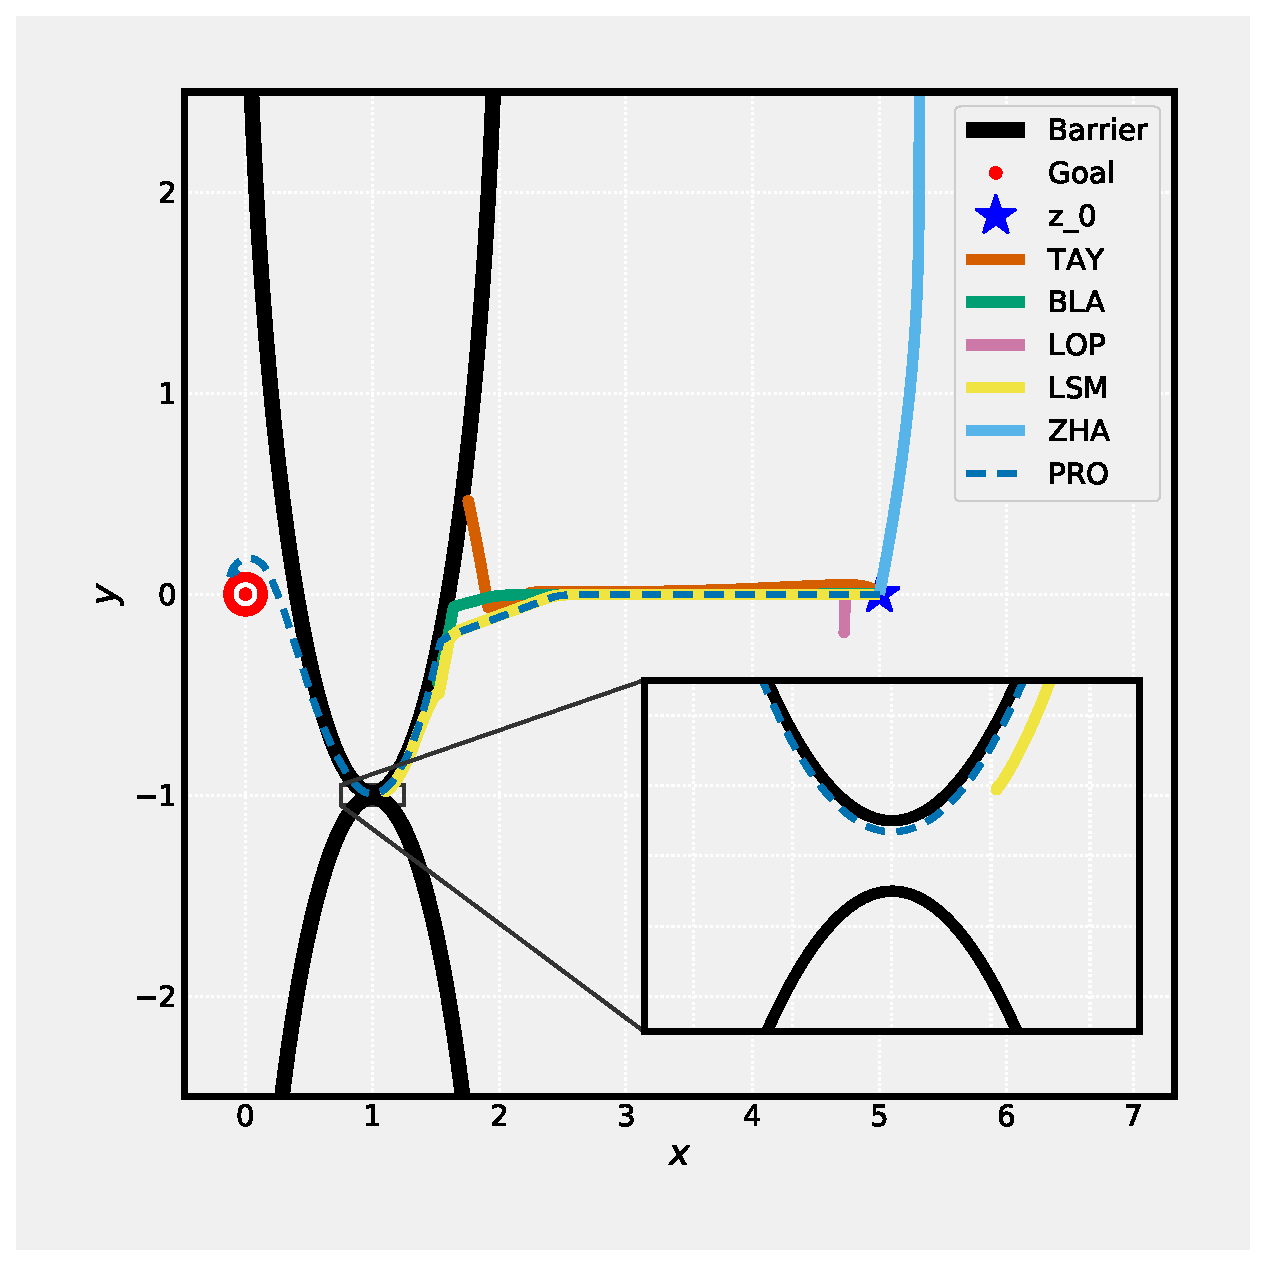
\includegraphics[width=0.33\textwidth,clip]{ShootTheGap_allFxTS_Trajectories.eps}
%         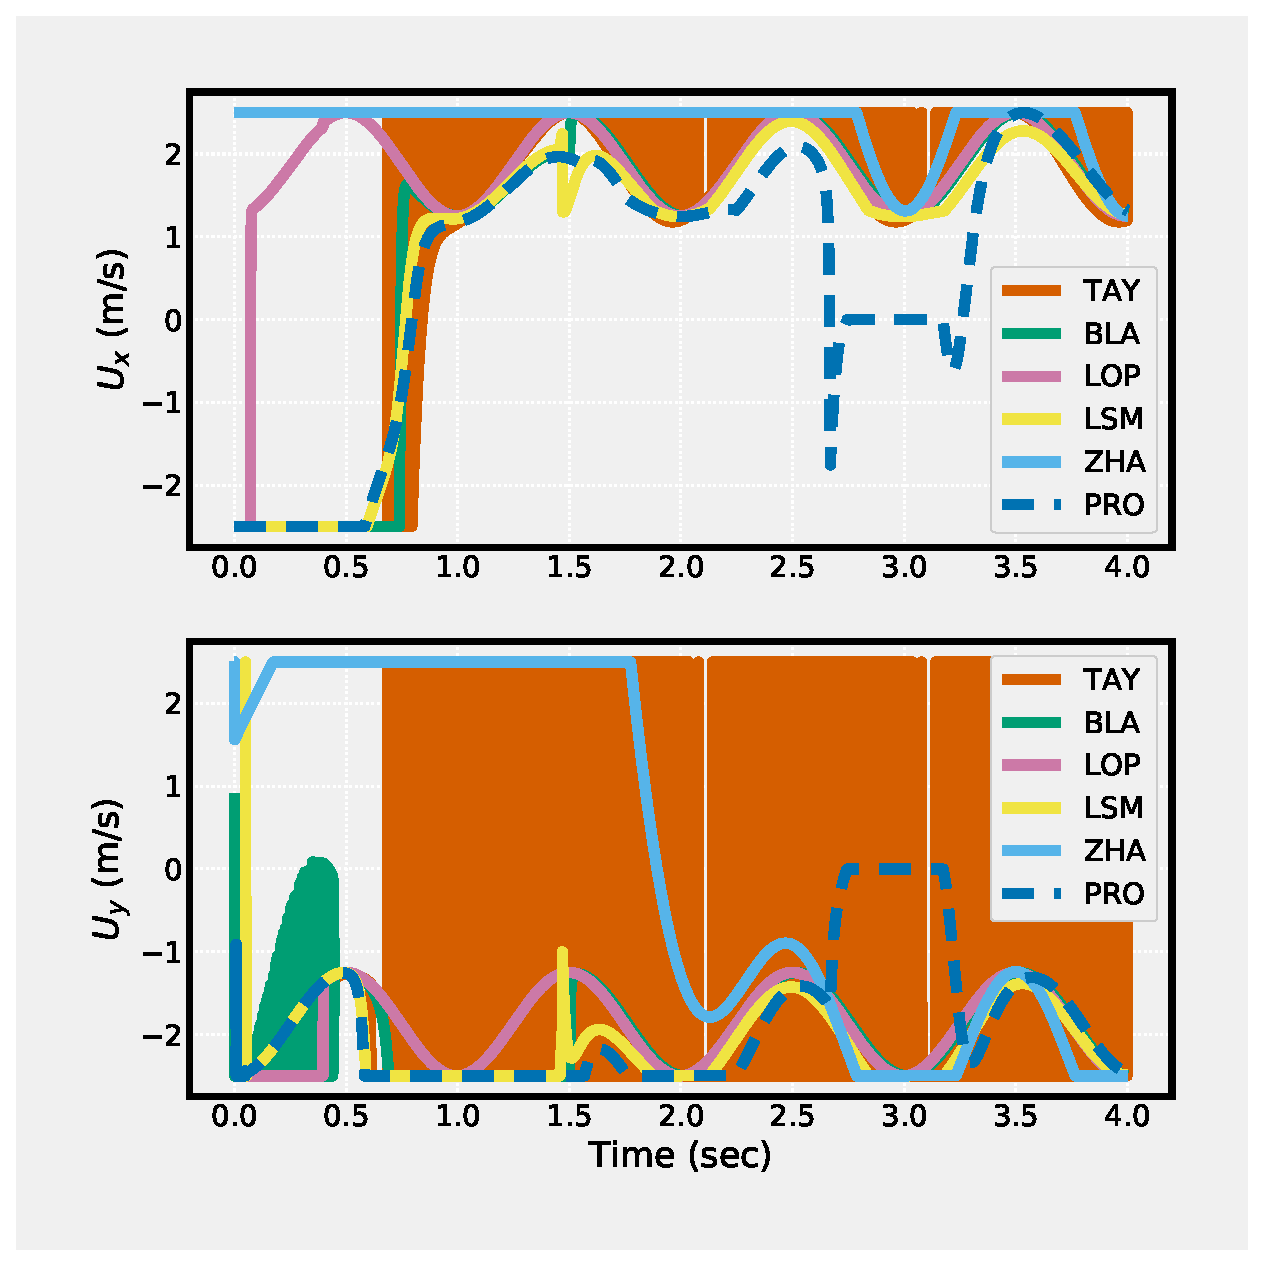
\includegraphics[width=0.33\textwidth,clip]{ShootTheGap_allFxTS_Controls.eps}
%         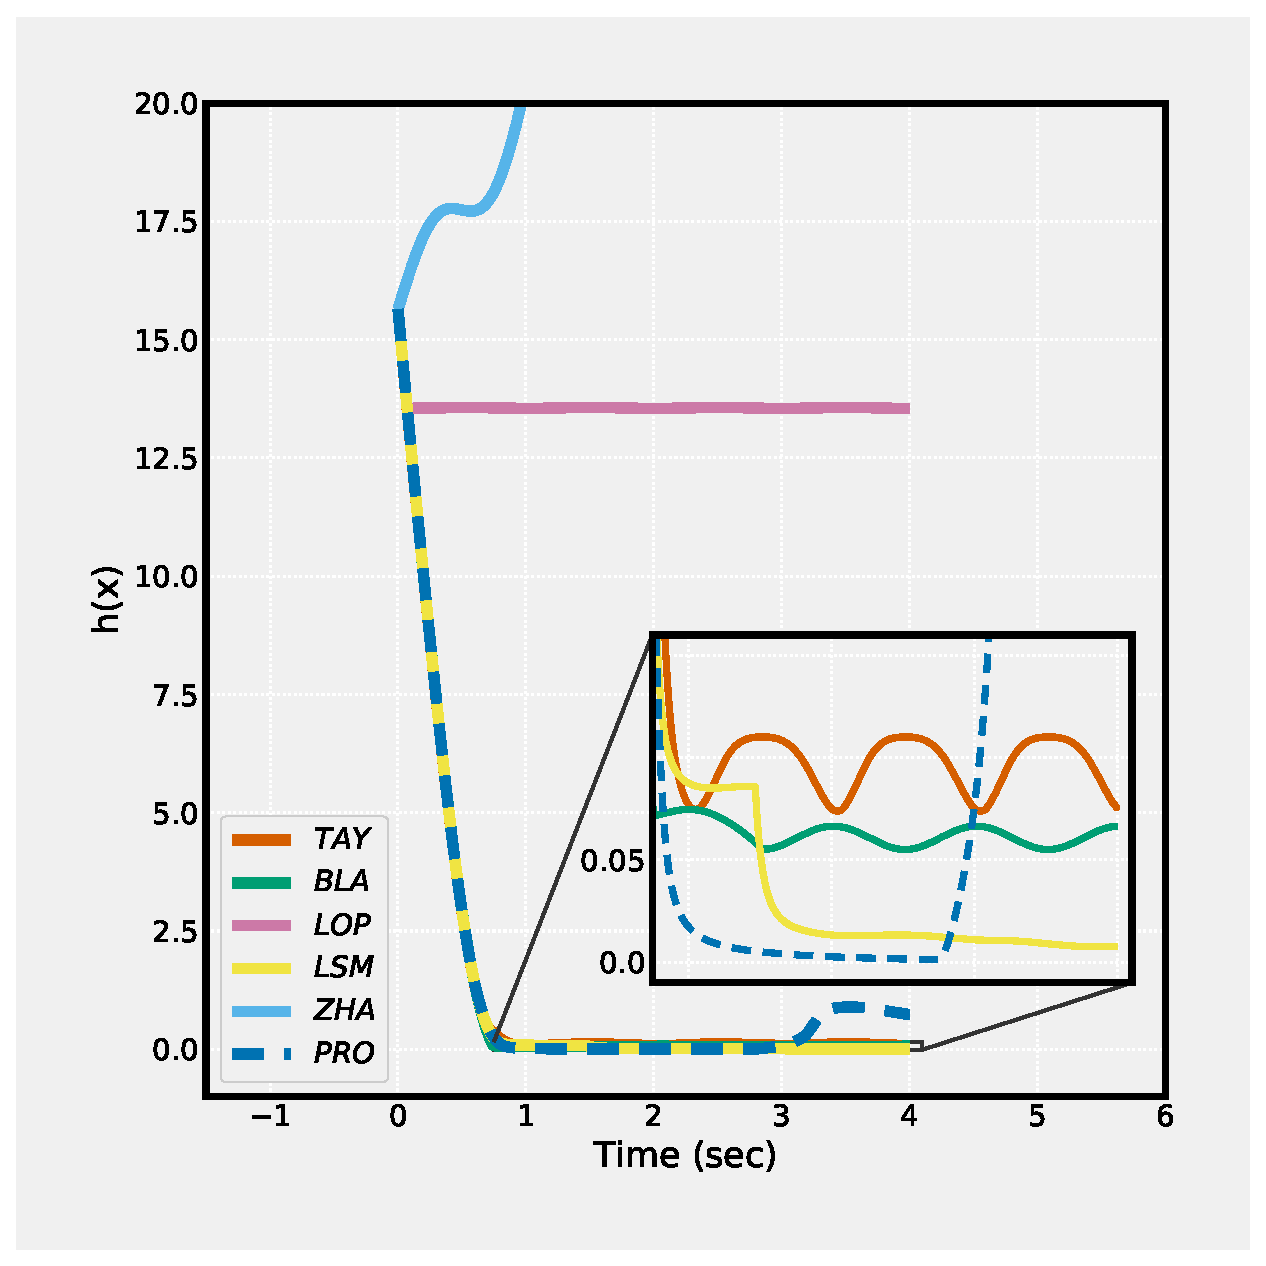
\includegraphics[width=0.33\textwidth,clip]{ShootTheGap_allFxTS_CBFs.eps}
%     \caption{Ego Vehicle trajectories, control inputs, and CLF / CBF evolution for 7 different initial conditions.}\label{fig: FxTS shoot the gap}
% \end{figure*}



% \begin{figure}[!ht]
%     \centering
%         \includegraphics[width=1\columnwidth,clip]{nominal_trajectories.eps}
%         \includegraphics[width=1\columnwidth,clip]{nominal_inputs.eps}
%         \includegraphics[width=1\columnwidth,clip]{nominal_CLFCBF.eps}
%     \caption{Ego Vehicle trajectories, control inputs, and CLF / CBF evolution for 7 different initial conditions.}\label{fig:2}
% \end{figure}

%%%%%%%%%%%%%%%%%%%%%%%%%%%%%%%%%%%%%%%%%%%%%%%%%%%%%%%%%%%%%%%%%%%%%%%%%%%%%%%%
%**************************** Numerical Case Study ****************************%
%%%%%%%%%%%%%%%%%%%%%%%%%%%%%%%%%%%%%%%%%%%%%%%%%%%%%%%%%%%%%%%%%%%%%%%%%%%%%%%%

\section{Highway Overtake}\label{sec: overtake}

In this section, we consider an automobile highway overtake problem, similarly to \cite{black2020quadratic}, and show how the proposed technique is capable of guaranteeing success of a safe overtake maneuver under uncertainty where the pure robust CBF approach is not.
% outperforms the worst-case, robust CBF approach in safely completing the overtake maneuver under uncertainty.

\subsection{Dynamics}

Just as in \cite{black2020quadratic}, we model the automobiles as kinematic bicycles using the model presented in \cite{Rajamani2012VDC}. Accordingly, the state vectors are $z_i = [x_i\;y_i\;\theta_i\;v_i]^T$, where $x$ and $y$ are planar Euclidean coordinates (longitudinal and transverse, respectively), $\theta$ is the heading angle, $v$ is velocity, and the subscript $i \in \{e,l\}$ denotes belonging to the Ego or Lead vehicles. The corresponding dynamical system is described by:
\small{
\begin{align}\label{eq: overtake_dynamics}
    \dot z_i = 
        \begin{bmatrix}
            v_i \ \cos(\theta_i) \\
            v_i \ \sin(\theta_i) \\
            0 \\  0
        \end{bmatrix}
        + 
        \begin{bmatrix}
            0 & 0 \\
            0 & 0 \\
            1 & 0 \\
            0 & 1 / M
        \end{bmatrix}
        \begin{bmatrix}
            \omega_i \\ a_i\end{bmatrix}+ \Delta_i(z)\theta,
\end{align}
}\normalsize

\noindent where $M$  is the mass of the vehicle in kg, and $\omega_i$ and $a_i$ represent the angular velocity and heading acceleration control inputs, for which the bounds $\ubar{\omega} \leq \omega_i \leq \bar{\omega}$ in rad$^{-1}$ and $\ubar{a} \leq a_i \leq \bar{a}$ in m/s$^2$ hold. For reference, all overtake parameter values may be found in Table \ref{table overtake params}.
% , where $\bar{\omega}=0.175$ rad$^{-1}$, $\ubar{\omega}=-\bar{\omega}$, $\bar{a}=4890.285$ m/s$^2$, and $\ubar{a}=-\bar{a}$. 
We elect to model erratic, or distracted, driver behavior by the addition of the uncertain term $\Delta_i(x)\theta$, where $\Delta_i: \mathbb{R}^{4} \rightarrow \mathbb{R}^4 \times \mathbb{R}^p$ is the known regressor matrix. As such, we let $\Delta_e = 0_{n \times p}$ and $\Delta_l = 0_{n \times p}$ with the exception of $\Delta_{l,(0,0)}(z) = 1 + \frac{1}{2}(1 - \cos(2\pi f_{l,1}x_l))$ and $\Delta_{l,(1,1)}(z) = \frac{1}{10} + \frac{1}{20}(1 - \sin(2\pi f_{l,2}x_l))$.

% \small{
% \begin{align}
%     \Delta_l(z) &= 
%     \begin{bmatrix}
%             1 + \frac{1}{2}(1 - \cos(2\pi f_{l,1}x_l)) & 0 \\
%             0 & \frac{1}{10} + \frac{1}{20}(1 - \sin(2\pi f_{l,2}x_l)) \\
%             0 & 0 \\
%             0 & 0 
%     \end{bmatrix}%,\\
%     % \phi_{oc} &= 
%     % \begin{bmatrix}
%     %         1 + \sin^2(2\pi f_{oc,1}t) & 0 \\
%     %         0 & 1 + \cos^2(2\pi f_{oc,2}t) \\
%     %         0 & 0 \\
%     %         0 & 0 
%     % \end{bmatrix}
% \end{align}
% }\normalsize

\subsection{Problem Formulation}

We define the following safe sets:

\begin{equation}
    S_i = \{z \; | \; h_i(z) \geq 0\}, \; \forall i \in \{1,2,3\}
\end{equation}
where
\begin{align}
    h_1(z) &= K_s\left((y_e - E_R(z))(E_L(z) - y_e) \right)\label{cbf road}\\
    h_2(z) &= L - v\label{cbf speed}\\
    h_3(z) &= \left( \frac{x_e - x_l}{s_{x}}\right)^2 + \left( \frac{y_e - y_l}{s_{y}}\right)^2 - 1\label{cbf car}
\end{align}
and
\small{
\begin{align}
    E_R(z) = e_r &+ \frac{\theta_ev_e\sin(\theta_e)}{\bar{\omega}} \nonumber \\
    &- \frac{\theta_e^2}{2\bar{\omega}^2}\left(\frac{\bar{a}\sin(\theta_e)}{M} + v_e\bar{\omega}\cos(\theta_e)\right)\label{edge1}\\
    E_L(z) = e_l &- \frac{\theta_ev_e\sin(\theta_e)}{\bar{\omega}} \nonumber\\
    &- \frac{\theta_e^2}{2\bar{\omega}^2}\left(\frac{\bar{a}\sin(\theta_e)}{M} - v_e\bar{\omega}\cos(\theta_e)\right)\label{edge2}
\end{align}}\normalsize
where $e_r$ and $e_l$ denote the physical edges of the right and left side of the road such that \eqref{edge1} and \eqref{edge2} imply that \eqref{cbf road} encodes that the Ego vehicle remain on the road despite bounded steering capabilities. We also have that \eqref{cbf speed} enforces the road speed limit in m/s, $L$, and \eqref{cbf car} ensures that safety margins $s_x = \tau v_e\cos(\theta_e) + l_c$ and $s_y = w_c + 0.75$ between vehicles are observed, where $l_c$ and $w_c$ are the length and width of the vehicles in m. Then, $S = \cap S_i$, $\forall i \in \{1, 2, 3\}$.

In addition, Oncoming vehicles are known to obey the following pattern: the first vehicle has a time-headway of 24s with the Lead Vehicle, and subsequent Oncoming vehicles arrive in 30s intervals. Consequently, the Ego vehicle must be able to complete the overtake within 24s to proceed at the outset, and within 30s to proceed after the first Oncoming vehicle passes. 

We now formally define the overtake problem.

\begin{Problem}
    Given the initial states, $z_e(0)$, $z_l(0)$, the time headway of an oncoming vehicle, $T_h$, and the set $\Theta$ to which the unknown parameter vector, $\theta$, belongs, determine whether it is safe for the Ego vehicle to overtake the Lead vehicle, i.e. whether there exist $z(t)$, $u_e(t) \in \mathcal{U} = \{(\omega_e, a_e) \; | \; \ubar{\omega} \leq \omega_e \leq \bar{\omega}, \; \ubar{a} \leq a_e \leq \bar{a}\}$ such that $z_e(t) \in S$, $\forall t \in [0,T]$, where $T$ is the upper bound on time to complete the overtake. If safe and $T \leq T_h$, design a control input, $u_e(t) \in \mathcal{U}$ for the given $z(0)$ such that the Ego vehicle overtakes the Lead vehicle.
\end{Problem}

% The problem is partitioned into four sub-problems in the following way through the use of waypoints:

% \begin{enumerate}\label{list: subproblems}
%     \item Ego Vehicle approaches Lead Vehicle
%     \item Ego Vehicle merges into overtake lane
%     \item Ego Vehicle advances beyond Lead Vehicle
%     \item Ego Vehicle merges back into original lane
% \end{enumerate}

\subsection{Control Formulation}

We use the CLF-CBF-QP control framework presented in \eqref{CLF-CBF QP} to compute the control inputs, $u_1=\omega_e$ and $u_2=a_e$, pointwise-in-time where $q=3$ in accordance with $h_1(z)$, $h_2(z)$, and $h_3(z)$ in \eqref{cbf road}-\eqref{cbf car}. We replace the more general \eqref{pt_S1} with our novel RaCBF condition \eqref{RaCBF Condition} as our safety constraint. Our CLF is:
\begin{equation}
    V(z) = K_V(k_x\bar{x}^2 + k_y\bar{y}^2 + k_\theta\bar{\theta}^2 + k_v\bar{v}^2 - 1)
\end{equation}
where $\bar{x}=x-x_d$, $\bar{y}=y-y_d$, $\bar{\theta}=\theta-\theta_d$, and $\bar{v}=v-v_d$, and $z_d = [x_d \; y_d \; \theta_d \; v_d]^T$ is the desired state. The fully specified parameter values may be found in Table \ref{table overtake params}\footnote{\label{mustang}$M$, $l_c$, and $w_c$ taken from \href{https://www.ford.com/cars/mustang/models/shelby-gt350r}{2020 Ford Mustang Shelby GT}}.

{\small
\begin{table}[h!]
    \setlength{\tabcolsep}{4pt}
    \centering
    \caption{Overtake Parameters}\label{table overtake params}
    \begin{tabular}{|c|c|c|c|c|c|c|c|c|c|}
        \hline
        $\dot{x}$ & Val & QP & Val & CBF & Val & CLF & Val & $\dot{\hat{\theta}}$ & Val \\ \hline
        $M$ & 1994 & $Q_{0,0}$ & 1/$\bar{\omega}^2$ & $e_r$ & 0 & $K_V$ & 10$^{-5}$ & $k_e$ & 0.001 \\ \hline
        $f_{l,1}$ & 0.01 & $Q_{1,1}$ & 1/$\bar{a}^2$ & $e_l$ & 6 & $\mu$ & 5 & $T_e$ & 0.2 \\ \hline
        $f_{l,2}$ & 0.02 & $p_0$ & 5$\times10^{8}$ & $L$ & 30 & $\gamma_1$ & 0.8 & $\mu_e$ & 5 \\ \hline
        $\theta_1$ & -1 & $p_1$ & 1 & $l_c$ & 4.81 & $\gamma_2$ & 1.2 & $c_{1e}$ & 50 \\ \hline
        $\theta_2$ & 0 & $p_2$ & 1 & $w_c$ & 1.92 & $k_x$ & 0.0625 & $c_{2e}$ & 50  \\ \hline
         & & $p_3$ & 1 & $\tau$ & 1.8 & $k_y$ & 100 & $c_{2e}$ & 50  \\ \hline
         & & $\bar{\omega}$ & 0.175 & & & $k_\theta$ & 400 & $\gamma_{1e}$ & 0.8  \\ \hline
         & & $\bar{a}$ & 4890 & & & $k_v$ & 1 & $\gamma_{2e}$ & 1.2 \\ \hline
         & & & & & & & & $\ell_e$ & 100\\
        \hline 
    \end{tabular}
    Note: $Q_{i,j}$ denotes the value of the row $i$ column $j$ entry for the $Q$ matrix. Non-specified entries are uniformly zero.
\end{table}
}

\subsection{Results}

\begin{figure*}[!h]
    \centering
        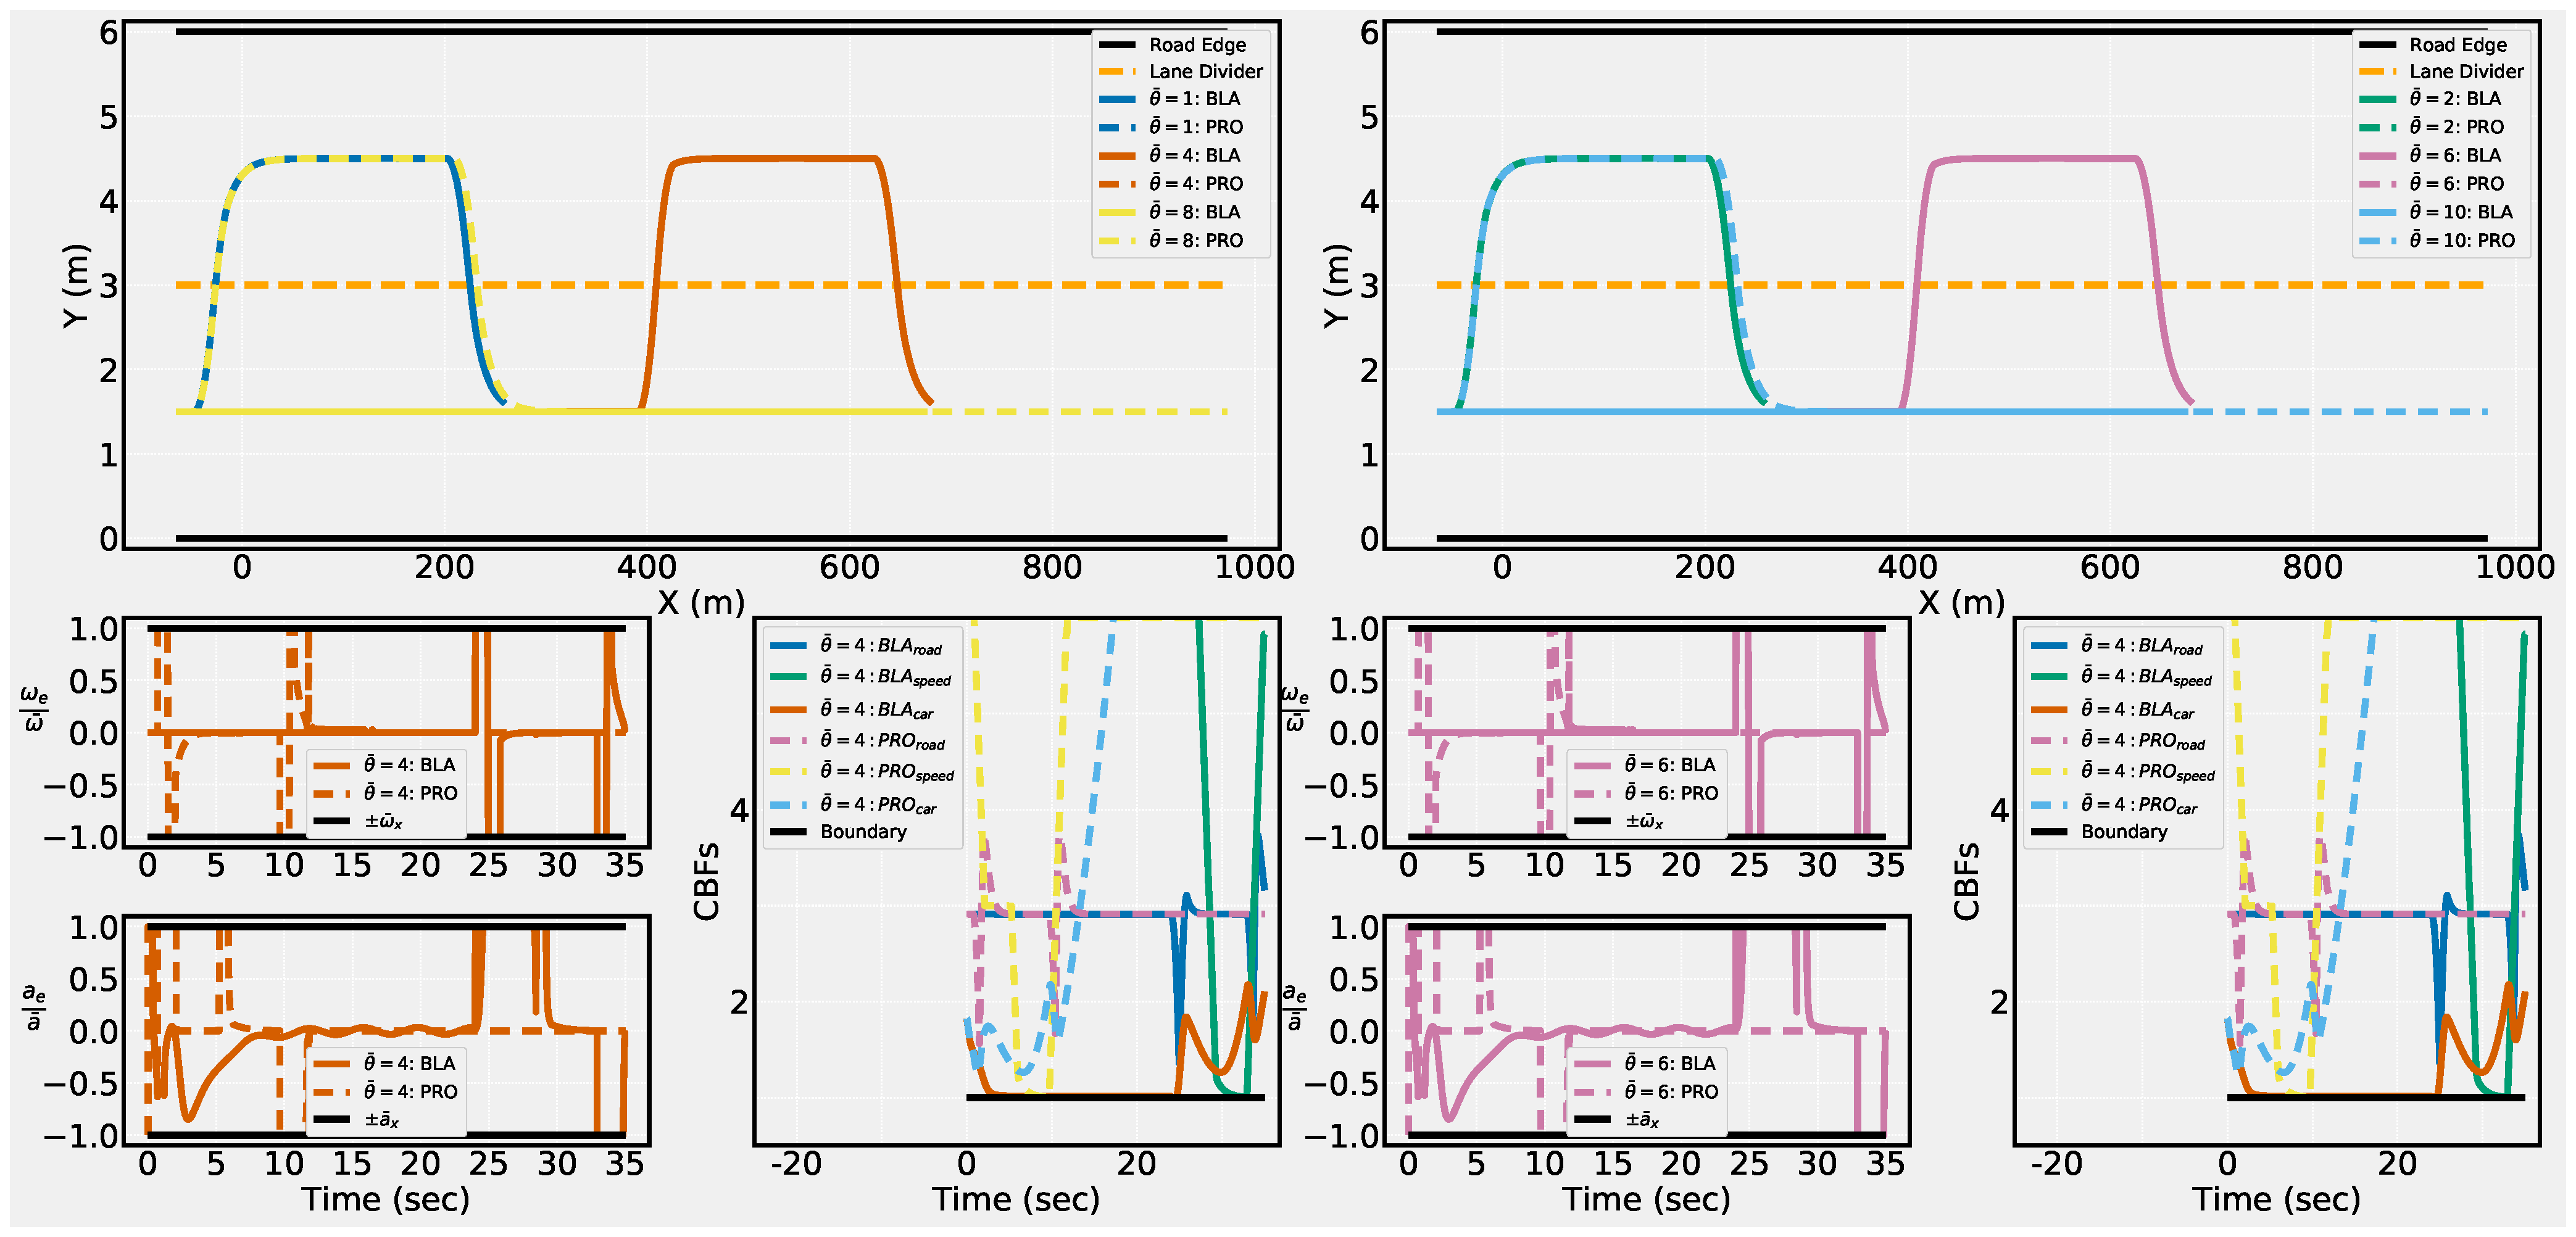
\includegraphics[width=1\textwidth,clip]{Overtake_AllPlots.eps}
    \caption{Numerical results for 6 different simulations of the overtake problem. In top row we display the state trajectories, including cases for which the proposed method successfully completes the overtake maneuver where the method developed in \cite{black2020quadratic} either must postpone the maneuver or cannot attempt it whatsoever. The bottom row contains two corresponding sets of control inputs and control barrier function trajectories for cases where \cite{black2020quadratic} must postpone the maneuver.} \label{fig: overtake}
\end{figure*}

The scenario was initialized as $x_e(0) = -64.8$, $y_e(0) = 1.5$, $\theta_e(0) = 0$, $v_e(0) = 24$, $x_l(0) = 0$, $y_l(0) = 1.5$, $y_\theta(0) = 0$, and $v_l(0) = 19$. For all considered sets of admissible parameters, $\Theta$, we set $\bar{\theta}_1 = -\ubar{\theta}_1 = \bar{\theta}_2 = -\ubar{\theta}_2$, and chose $\bar{\theta}_1 = 1, 2, 4, 6, 8, 10$ in succession.
% ,  $z_e(0) = [-64.8 \; 1.5 \; 0 \; 24]^T$ and $z_l(0) = [0 \; 1.5 \; 0 \; 19]^T$

The component-wise upper and lower bounds on the admissible set of parameters, $\Theta$, were varied for the same set of initial conditions. As $\Theta$ grows, so does the uncertainty in the system dynamics. Because the proposed method is guaranteed to adaptively learn the true parameters within fixed-time, it is able to successfully complete the overtake maneuver for all considered sets, $\Theta$. While Figure \ref{fig: overtake} highlights this capability, it also illustrates the limitations of the method proposed by \cite{black2020quadratic}. As the bounds on the uncertain parameters increase, that controller is unable to guarantee FxT convergence to the goal before the arrival of the Oncoming vehicle.

The fixed-time horizon required for the method proposed by \cite{black2020quadratic}, however, grows with the uncertainty.

% \begin{figure*}[!ht]
% % \begin{mdframed}[backgroundcolor=#1]
% \hspace*{-1.25em}
% \begin{subfigure}{0.35\linewidth}
%     % \centering
%     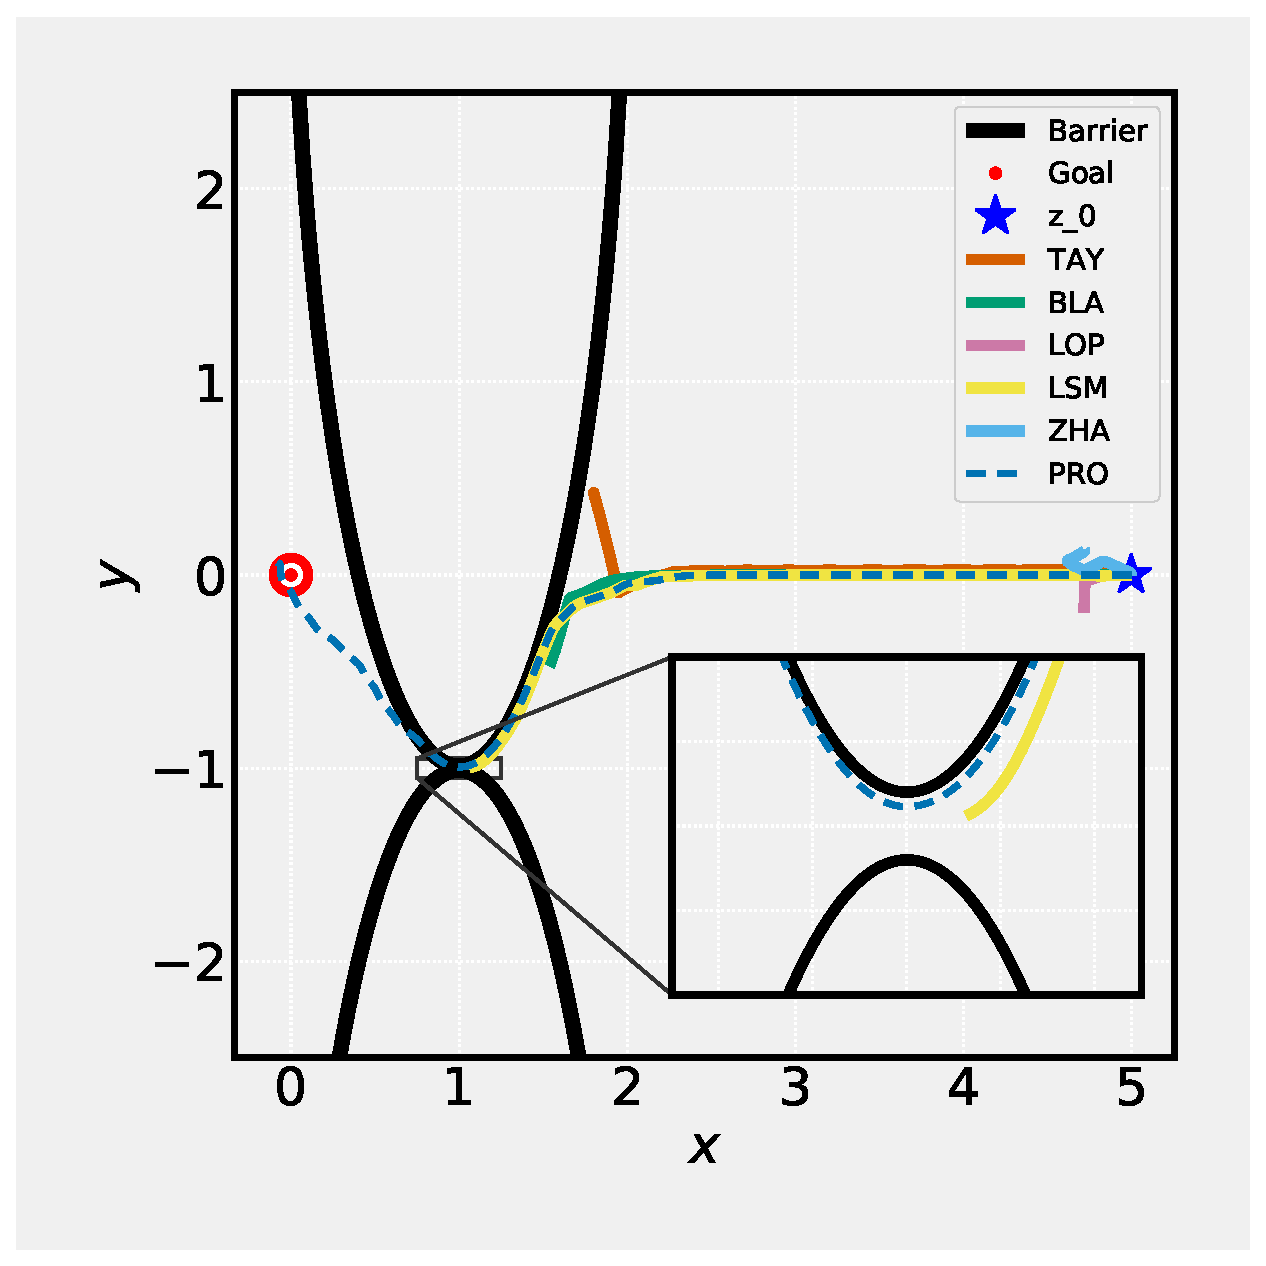
\includegraphics[width=1\textwidth,left]{ShootTheGap_allFxTS_Trajectories_RegX.eps}
%     \caption{State trajectories}\label{fig: FxTS shoot the gap - trajectories}
% \end{subfigure}%
% \hspace*{-0.25em}
% \begin{subfigure}{0.35\linewidth}
%     % \centering
%     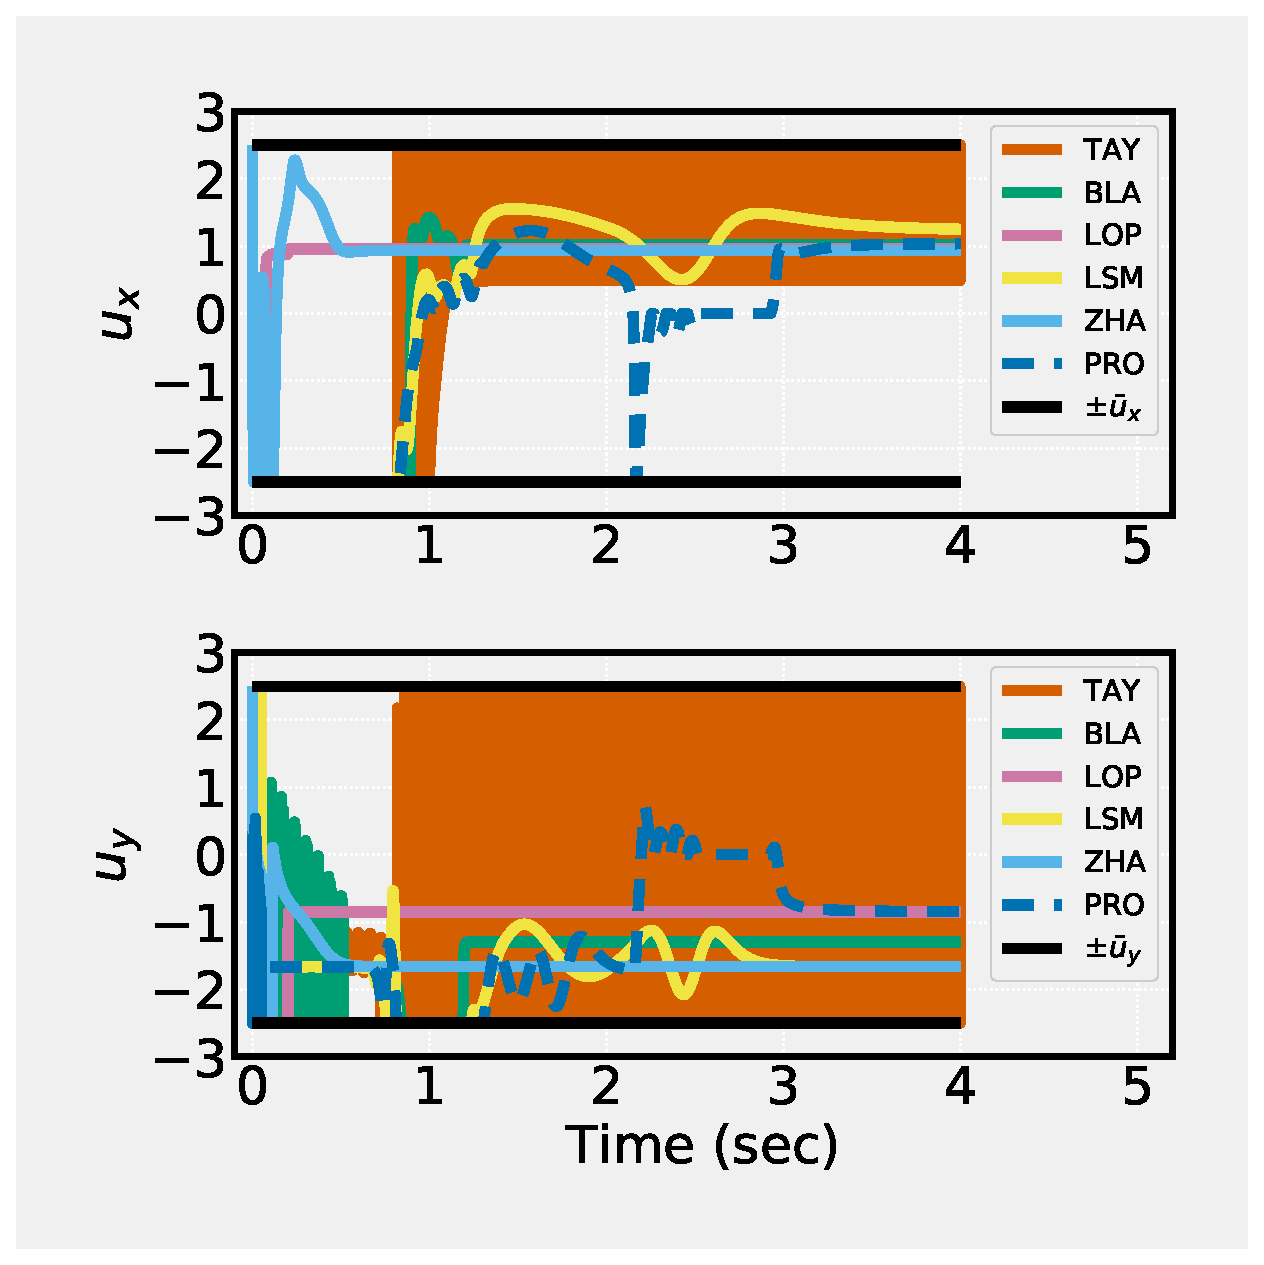
\includegraphics[width=1\textwidth]{ShootTheGap_allFxTS_Controls_RegX.eps}
%     \caption{Control inputs}\label{fig: FxTS shoot the gap - controls}
% \end{subfigure}%
% \hspace*{-0.25em}
% \begin{subfigure}{0.35\linewidth}
%     % \centering
%     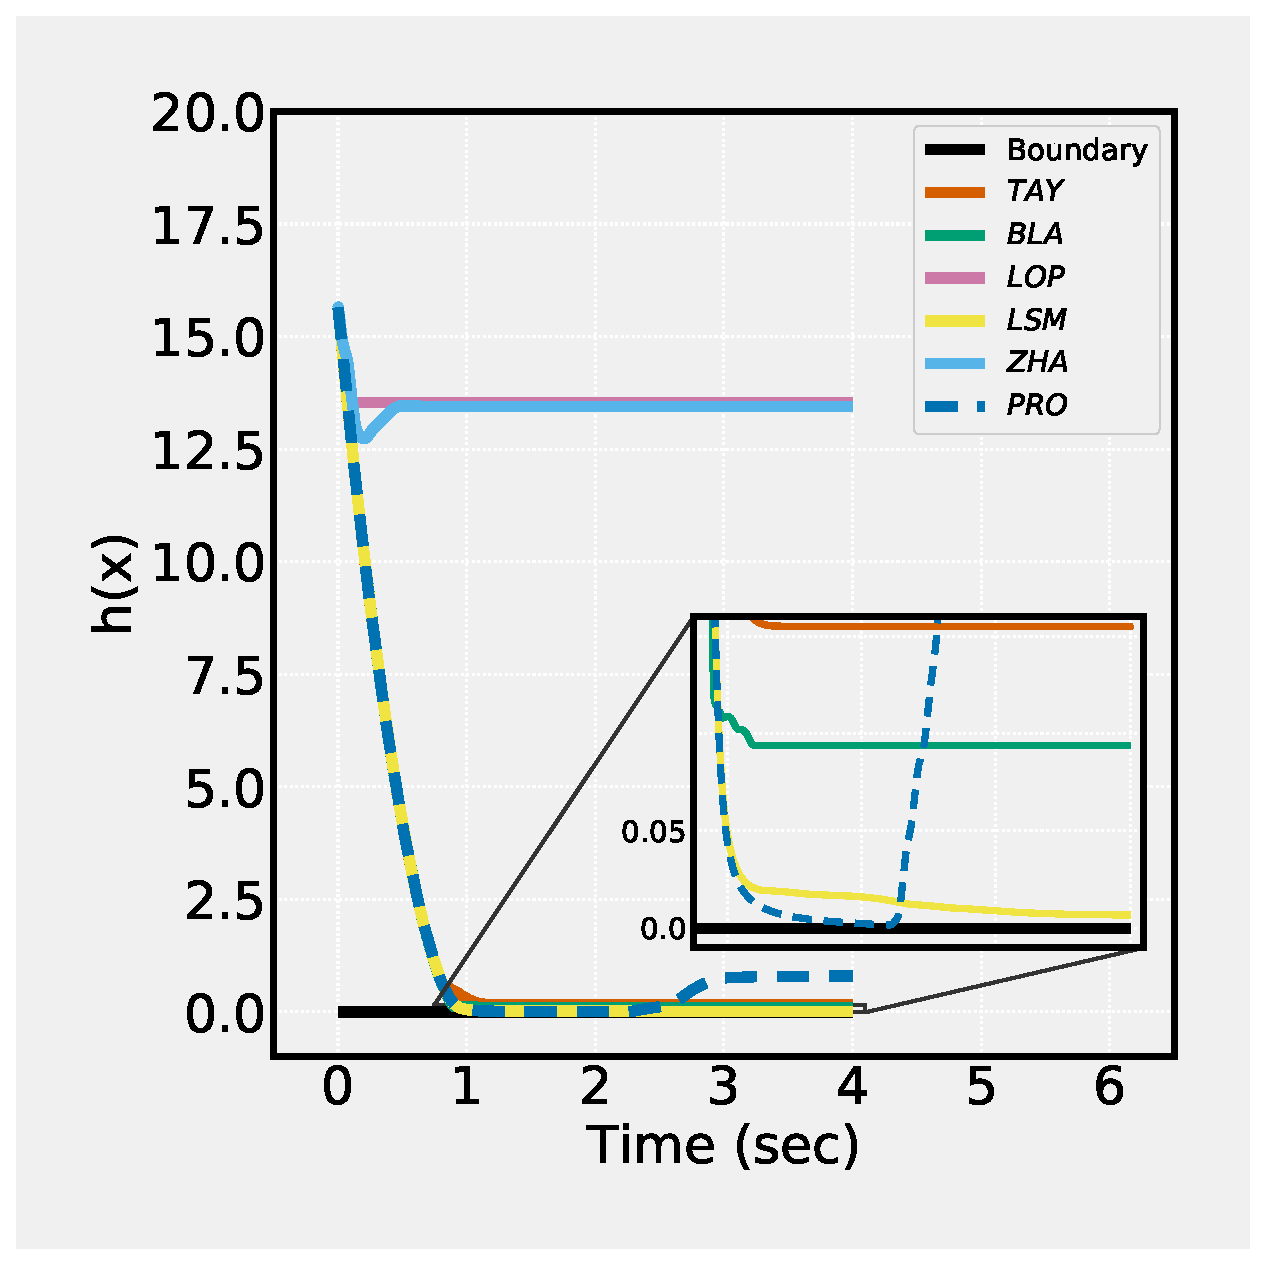
\includegraphics[width=1\textwidth,right]{ShootTheGap_allFxTS_CBFs_RegX.eps}
%     \caption{Value of level curve for safe set}\label{fig: FxTS shoot the gap - cbfs}
% \end{subfigure}%
% \caption{State trajectories, control inputs, and control barrier function evolutions in time for the Shoot the Gap example.}
% % \end{mdframed}
% \end{figure*}
%%%%%%%%%%%%%%%%%%%%%%%%%%%%%%%%%%%%%%%%%%%%%%%%%%%%%%%%%%%%%%%%%%%%%%%%%%%%%%%%
%********************************* Conclusion *********************************%
%%%%%%%%%%%%%%%%%%%%%%%%%%%%%%%%%%%%%%%%%%%%%%%%%%%%%%%%%%%%%%%%%%%%%%%%%%%%%%%%

\section{Conclusion}
 In this study on the efficacy of various techniques for safe control under parametric model uncertainty, we presented a novel method for adaptively learning the structured uncertain parameters associated with the model of a dynamical system in fixed-time. We synthesized our parameter adaptation law with a robust, adaptive control barrier function based controller in the form of a quadratic program, and provided an upper bound on the parameter estimation error as an explicit function of time so as to guarantee safety at all times. We then studied the performance of our method on a simple, 2D single integrator system in relation to several recent works from the literature and demonstrated that our contribution succeeds in navigating near unsafe regions where the others fail. We further illustrated the promise of our method in applications where a decision on whether to initiate a possibly unsafe maneuver is required, using the automobile highway overtake problem as a case study.

In the future, we intend expand the realm of consideration to include both the cases where the uncertain parameters are time-varying and when an upper bound is not known a priori, as we recognize that these may have broader applicability to real-world scenarios.

%%%%%%%%%%%%%%%%%%%%%%%%%%%%%%%%%%%%%%%%%%%%%%%%%%%%%%%%%%%%%%%%%%%%%%%%%%%%%%%%
%*********************************** Errata ***********************************%
%%%%%%%%%%%%%%%%%%%%%%%%%%%%%%%%%%%%%%%%%%%%%%%%%%%%%%%%%%%%%%%%%%%%%%%%%%%%%%%%

% \subsection{Estimate of Allowable Initial Subset of Safe Set}

% We now discuss an estimate, albeit conservative, of the safe initial states, $x_0$, for a class of dynamical systems described by \eqref{uncertain system}. First, we review the set of local Lipschitz continuity assumptions imposed on $f$, $g$, and $\Delta$.

% \begin{Assumption}\label{Lipschitz continuity}
%     Each of $f$, $g$, $\Delta$, and $h$ are piecewise continuous in $t$ and locally Lipschitz in $x$, that is:
%     \begin{itemize}
%         \item $\|f(t,x) - f(t,y)\| \leq F\|x-y\|$
%         \item $\|g(t,x) - g(t,y)\| \leq G\|x-y\|$
%         \item $\|\Delta(t,x) - \Delta(t,y)\| \leq D\|x-y\|$
%         \item $\|h(t,x) - h(t,y)\| \leq H\|x-y\|$
%     \end{itemize}
%     for all $x,y \in S = \{x \in \mathbb{R}^n: h(x) \geq 0\}$.
% \end{Assumption}

% \begin{Remark}
%     We observe that an implication of Assumption \ref{Lipschitz continuity} is that for every initial condition belonging to the interior of the safe set, i.e. $\forall x_0 \in int(S)$, there exists a ball of radius $r$, $B = \{x \in S: \|x-x_0\| \leq r\}$, such that each of the Lipschitz conditions hold.
% \end{Remark}

% However, we must also assume specific conditions on the set $S$, as follows:

% \begin{Assumption}
%     For every initial state, $x_0$, inside the safe set, $S$, there exists a ball of radius $r$ such that 
% \end{Assumption}

% \begin{equation}
%      \|h(x(T)) - h(x(0))\| \leq HTK
% \end{equation}

% where 

% \begin{equation}
%      K = Fr + \varphi + Gr\|u\|_{\infty} + \gamma \|u\|_{\infty} - Dr\|\theta\|_{\infty} - \delta \|\theta\|_{\infty}
% \end{equation}


% where $z_e$ denotes the state of the ego agent (the subject-agent for which the controller, $u$, is designed), $z_i$ for $i \in [1,N]$ denotes the state of the $i$th agent, $\phi _i$ is a vector of unknown parameters belonging to a nonlinearly parameterized dynamical model for agent $i$, $N$ is the number of agents under consideration, $y_k$ represents the set of state measurements for all agents collected at time $t_k$\iffalse, and $v(t)$ is a zero-mean, white, stationary, Gaussian noise term\fi. We assume also that $f_e: \mathbb{R}^n \rightarrow \mathbb{R}^n$ and $f_i: \mathbb{R}^n \rightarrow \mathbb{R}^n$ for all $i \in [1,N]$ are locally Lipshitz.

% Due to the demonstrated efficacy [sources] of the synthesized CLF-CBF-QP control formulation in providing performance guarantees while observing forward-invariance of a safe set, we employ this framework for the purpose of our controller design in the following discussion.

% \subsection{Parameter Estimation}
% We now address the problem of estimating the unknown parameters belonging to $\phi \in \mathbb{R}^m$. The proposed technique relies on the method of nonlinear multivariate regression. Before proceeding, we need to establish the following assumptions.

% \begin{Assumption}
% Our ego agent has access to perfect state measurements at discrete time intervals through the measurement model, $y_k$.
% \end{Assumption}

% \begin{Assumption}
% The nonlinearly parameterized model uncertainty belongs to a compact domain, $\phi _i \in \Phi$.
% \end{Assumption}

% By employing these assumptions, we may estimate the unknown parameters present in the nonlinear dynamical models by solving a nonlinear multivariate regression problem of the following form:

% \begin{subequations}\label{Parameter Estimation Regression}
% \begin{align}
%     \hat{\phi} = \argmin \frac{1}{2} \|\hat{\mu} - \mu (y_{1,...,k},\hat{\phi})\| \label{nl mult reg}\\
%     \textrm{s.t.} \; \hat{\phi} &\in \Phi \label{compact}
% \end{align}
% \end{subequations}

% where $\mu$ represents the estimated time-history of the dynamics to which the estimated parameters, $\phi$, are being fit.
% {\color{blue}
% \subsection{New Result on CBF with Parameterized Uncertainty}

% Consider the following CBF:

% \begin{equation}
%     h(x) = h_0(x) + \Omega(x)\phi
% \end{equation}

% \noindent where now $\phi$ is the vector of unknown parameters. The necessary and sufficient condition for forward-invariance of a safe set defined by $h$ then becomes:

% \begin{equation}
%     \dot{h}(x) = \frac{\partial h_0}{\partial x}\dot{x} + \frac{\partial \Omega}{\partial x}\phi\dot{x} \geq 0, \; \forall x \in \partial S
% \end{equation}

% \noindent We can rewrite $\dot{h}$ as a nonlinear dynamical system in the form of \eqref{Na uncertain system}, with $\varphi(x,u) = \frac{\partial h_0}{\partial x}\dot{x}$, and $\Phi(x,u) = \dot{x}^T\frac{\partial \Omega}{\partial x}$. We can then define $\dot{h}_f = \varphi_f(x,u) + \Phi_f(x,u)\phi$, where $\varphi_f(x,u) = \frac{\partial h_0}{\partial x}\dot{x}_f$, and $\Phi_f(x,u) = \dot{x}_f^T\frac{\partial \Omega}{\partial x}$, and use the auxiliary and integrated regressor matrix $P$ and vector $Q$ as in \eqref{filter P} and \eqref{filter Q} respectively to estimate the unknown parameter vector $\phi$ in fixed-time.}

\bibliographystyle{IEEEtran}
\bibliography{myreferences}


%%%%%%%%%%%%%%%%%%%%%%%%%%%%%%%%%%%%%%%%%%%%%%%%%%%%%%%%%%%%%%%%%%%%%%%%%%%%%%%%
%********************************* Appendices *********************************%
%%%%%%%%%%%%%%%%%%%%%%%%%%%%%%%%%%%%%%%%%%%%%%%%%%%%%%%%%%%%%%%%%%%%%%%%%%%%%%%%

% \appendices
% \section{Proof of Something}
% App. 1.





\end{document}